\documentclass[11pt]{jsreport}%article??

\usepackage{mypackage}


\newif\iffigure
%\figurefaulse
\figuretrue
%select show the figure or not

\makeatletter
\def\@cite#1{\textsuperscript{#1)}}
\def\@biblabel#1{#1)}
\makeatother

\newcommand{\DATE}[3]{#1年#2月#3日} %month, day, year
\newcommand{\TheDay}{\DATE{2020}{11}{30}}
%ヘッダとかもなくてもいいかも
%\newcommand{\Header}{中須賀・船瀬研究室}

\title{卒業論文} %最終発表
\date{\TheDay}
\author{
03-183005 西本 慎吾%\thanks{shingo_n@space.t.u-tokyo.ac.jp}
}

%ヘッダの指定:
\pagestyle{fancy}

%ここをtrueにすると全ビルド?ではないみたい
\newcommand{\ifdraft}{true}

\begin{document}
%\maketitle
%\thispagestyle{fancy}
%\lhead[\Header]{\Header} % ヘッダ左側
%\chead[偶数ページの引数]{奇数ページの引数} %ヘッダ中央
%\rhead[\TheDay]{\TheDay} %ヘッダ右側
%\lfoot[偶数ページの引数]{奇数ページの引数} %フッタ左側
%\cfoot[偶数ページの引数]{奇数ページの引数} %フッタ中央
%\rfoot[偶数ページの引数]{奇数ページの引数} %フッタ右側
\begin{titlepage}
  \begin{center}
  \vspace*{10zh}
  {\LARGE 東京大学工学部航空宇宙工学科\\令和2年度学士論文}
  \vspace{2zh} \\
  {\huge 衛星内の情報伝達経路モデルに基づく\\不具合分析支援に関する研究}
   \vspace{20zh} \\
   {\Large 03-183005 西本 慎吾}\\
   {\Large 指導教員 船瀬 龍 准教授}\\
   {\Large \TheDay}
  \vspace{12pt} \\
  \end{center}
\end{titlepage}


%あとでincludeからinputに戻すかな
%\include{abtract.tex}
%\include{abtract.tex}
\expandafter\ifx\csname ifdraft\endcsname\relax
\documentclass[11pt]{jsreport}
\usepackage{mypackage}
\begin{document}
\fi

\chapter{序論}
\section{研究背景} 
\subsection{超小型衛星の信頼性の低さ}
近年,超小型衛星の開発が大学や小企業の中で盛んになってきている.
これまでは教育目的が主であったが,商用利用や革新的なミッションへの応用も
増えてきている\cite{Langer2016}.
一方で現状の超小型衛星は中・大型衛星と比較して軌道上での不具合の確率は高く,
2002から2016の間に打ち上がった
270のCubesatのうち,139のミッションが失敗している\cite{Langer2016}.\\
大学衛星は宇宙環境での使用を保証されていない
民生部品を使用することも多いため,このような超小型衛星で頻発している
不具合は,軌道上での部品の故障によって発生すると考えられてきた.しかし,
実際には多くが設計や製造過程に起因する
%故障分析の意味
不具合であることが故障分析を通じて知られている\cite{Venturini2017}.
軌道上での不具合の根本原因に対する調査(図\ref{fig:cause of failure})では,
民生部品の品質の不確定性が原因であったものはわずか17%であり,
それ以外の多くが,設計や地上試験の不足に起因するものであることが
分かっている\cite{Venturini2017}.

%ここにできれば具体的な衛星の故障の例を持ってくれると良い
%論文で
\begin{figure}[H]
   \centering
      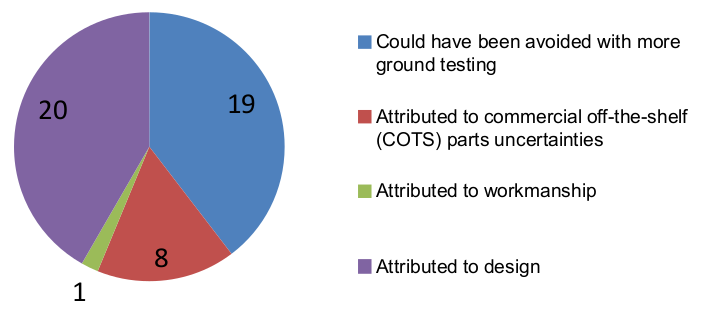
\includegraphics[height=4.5cm]{figure/cause_of_failure.png}
      \caption{故障原因に関するインタビュー結果\cite{Venturini2017}}
      \label{fig:cause of failure}
\end{figure}

%ここへのつながり.別subsectionのほうがいいかも
%ほどよし信頼性工学のところをしっかりとまとめたほうがいい
また,大学衛星が商用利用や革新的なミッションに
挑戦するためには,超小型衛星のメリットである
コストの低さを十分に確保しながら,ほどほどの信頼性
を実現する「ほどよし」の考え方が
重要であると考えられている\cite{SHIRASAKA2011}.\\
故障に設計や製造の不良が含まれていることを考えると,
超小型衛星のほどほどの信頼性の評価を行うためには,
従来用いられてきた
各コンポーネントごとの信頼度の組み合わせでは不十分である.
そこで,設計・製造・運用における
信頼度を加味した評価手法が提案されている\cite{SHIRASAKA2011}.
式(\ref{eq:Reliability})が示すように,この評価手法では
設計や製造時の信頼性も重要な要素であると捉えられている.\\
超小型衛星のコストの低さを考慮すると,信頼性の高いコンポーネントを使用することによって
それぞれのコンポーネントの信頼性$R_{comp}$を高めるより,
設計や製造過程における信頼性を高めることが超小型衛星の信頼性の向上につながる.
また上述したように,超小型衛星の信頼性の低さの根本原因である設計不良や地上試験の不足
を改善していくことが,信頼性向上には不可欠である.

\begin{equation}
   R_{sat} = R_{des} \times R_{fab} \times R_{comp} \times R_{op} \label{eq:Reliability}
\end{equation}
\begin{table}[H]
   \centering
      \begin{tabular}{cl} 
        $R_{sat}$ & 衛星の真の信頼度\\
        $R_{des}$ & 設計における信頼度\\
        $R_{fab}$ & 製造における信頼度\\
        $R_{comp}$ & 衛星の信頼度(従来の信頼度)\\%コンポーネントの信頼度
        $R_{op}$ & 運用における信頼度
      \end{tabular}
\end{table}
%これを言うことで,この研究ではこれらのどこを高めているのかを考える必要がある.

%もうちょいちゃんと考える
\subsection{地上試験における問題}
以上で示したように,不具合の多くが設計,製造などに起因しているという問題がある.
一方で,これは超小型衛星開発のみに限られたことではなく,
中・大型衛星においても大きな問題となっている.
軌道上故障データを分析した結果\cite{SAITO2011}(図\ref{fig:error type})
によると,軌道上で
偶発的に発生した故障はわずか11%であり,それ以外は設計,製造などの開発
活動に起因するものであることが分かっている.\\
また,軌道上で発生した不具合が「地上試験で
発現しなかった,または発見できかった原因」が以下の
図\ref{fig:error cause}のように知られている.
試験設備の不足によって確認できなかったものや,故障発見までの
時間が長く地上試験で発見することが現実的で無いものに関しては,
コストとリソースの面から試験による対策では限界がある.
一方で,試験モードの不備や,地上試験で発現していたのにもかかわらず
発見できなかった不具合に関しては試験に対する習熟度が不足していること,
不具合・リスクの分析が不十分であることが推測される\cite{SAITO2011}.

\begin{figure}[H]
   \centering
      \begin{tabular}{c}
         \begin{minipage}{0.50\hsize}
         \centering
         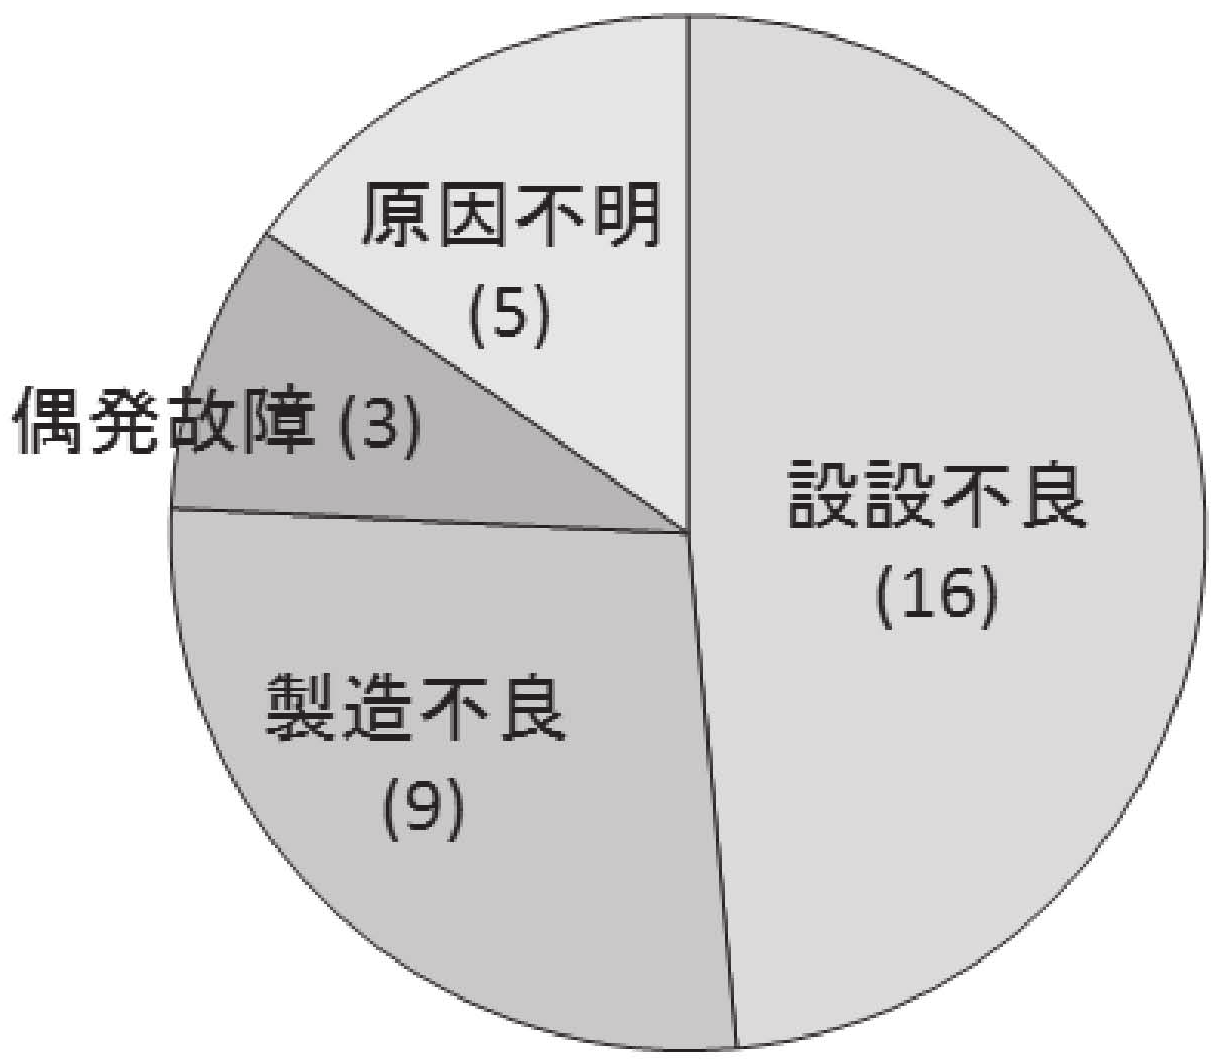
\includegraphics[width=5.5cm]{figure/on_orbit_error_tyoe.png}
            \caption{軌道上故障の原因類型の分布\cite{SAITO2011}}
            \label{fig:error type}
         \end{minipage}
         \begin{minipage}{0.50\hsize}
         \centering
         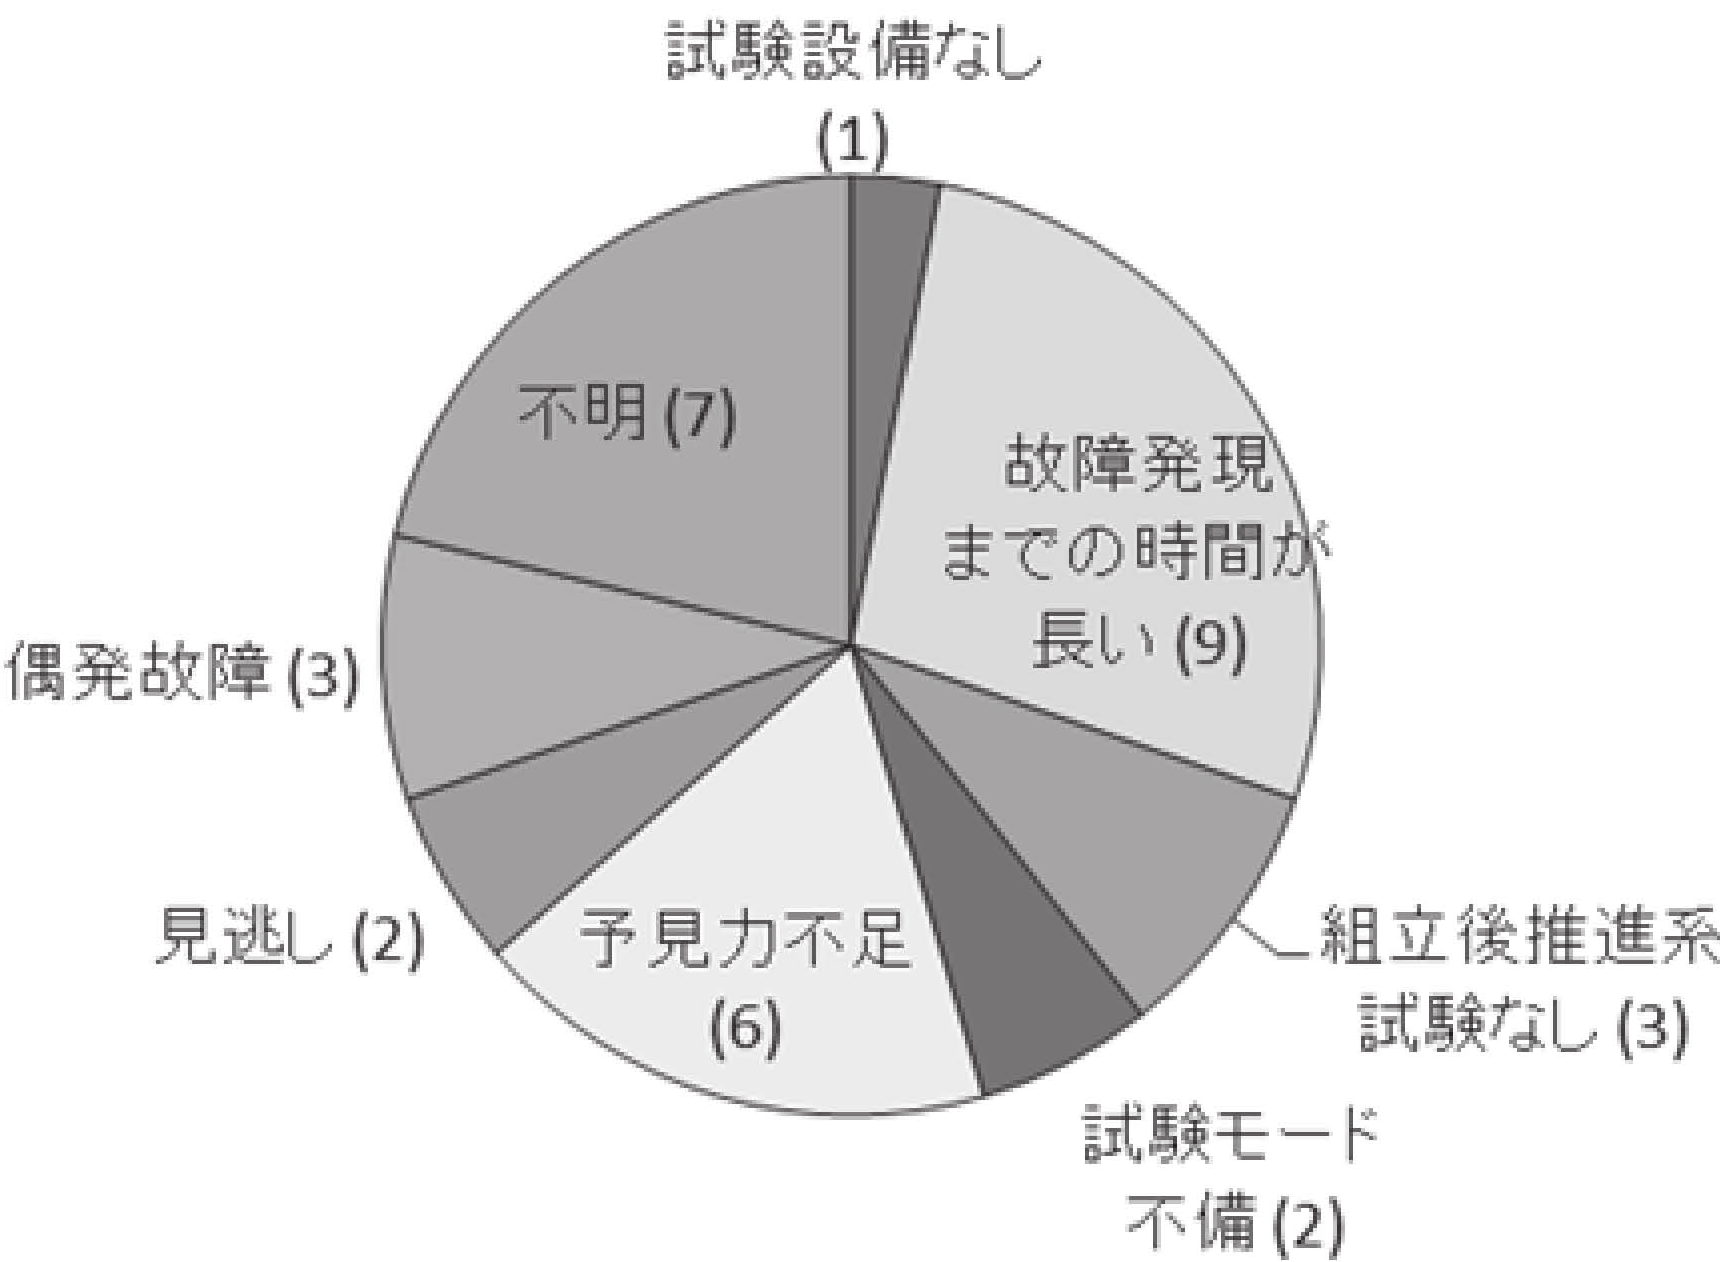
\includegraphics[height=5.5cm]{figure/not_found_error_seeds.png}
            \caption{軌道上故障の要因を地上で発見できなかった原因類型の分布\cite{SAITO2011}}
            \label{fig:error cause}
         \end{minipage}
      \end{tabular}  
\end{figure}

%ここに大学衛星の不具合分析に関する話があったような・・・・論文まとめから探し出せ

%ここの流れを見直す.根拠資料
\subsection{不具合原因特定の難しさ}
以上のように,衛星の不具合及びリスクの分析を,地上試験で十分に
行えていないことが,超小型衛星の信頼性の低さの原因の一つである.\\
そこで,地上試験で衛星の不具合及びリスク分析が十分に行えていない原因
を具体的に示すため,以下に人間による不具合分析の大まかな流れを示す.
\begin{enumerate}[1)]
   \item 不具合が起きた際の衛星の状態を保存し記録に残す. 
   \item テレメトリから考えられる故障原因の候補を洗い出す.
   \item それらの故障の中でテレメトリから分かる情報を元に候補を棄却していく.
   \item 更に切り分けが必要な場合はコマンドを送り,
   それに対するテレメトリの挙動によって判断するという作業を繰り返す.
   \item 判断できない場合は,コンポーネントを取り出し直接確認を行う.
\end{enumerate}
まず,地上試験において十分に不具合分析が行えていない原因の1つとして,2)の故障原因の候補
の洗い出しを網羅的に行うことの難しさがある.\\
組み上げ状態の衛星から得られる情報は主にテレメトリのみである.
この際,衛星の内部状態を理解し,テレメトリから現在の衛星の状態
を類推することができなければ,十分に不具合原因の候補を洗い出すことはできない.
また,衛星のように内部の機器が複雑に絡み合ったシステムでは,
人間が想定していないつながりが多数存在するため,不具合事象から全ての
故障可能性を洗い出すことは難しい.
本研究室の過去プロジェクト(PRISM)を対象にした研究では,
事前に想定していた故障モードの粒度は,%故障モードの意味
%ここの記述も微妙なので変更する
山口ら\cite{Yamaguchi2014}が構築したシステム
を用いて洗い出した故障モードと比較して,不足しているという結果も出ている.
このように,人間による故障モードの洗い出しは思いつきによるものなので,
人の知識や経験に依存し,考えが及んでいないことで見逃している故障モード
が多く存在する.

また,分析が不十分になっているもう一つの原因として,
3),4)の故障原因の切り分け作業の難しさがある.\\
上述したように超小型衛星は内部状態が複雑に絡み合っており,一つの不具合に対して
非常に多くの故障候補が洗い出される.
%切り分けを行うためのコマンドを探すのが難しい
そのため,多くの故障候補の中から切り分けを行い,最終的な故障を
特定するという作業は多くの知識と労力を必要とする作業である.
また,実ミッションで使用するコマンドとテレメトリは膨大な数であるため,
その中から切り分けを行うための情報を選択し,仮説の検証を行う作業は
無駄やヒューマンエラーを生むきっかけとなる.
不具合発生時は衛生の状態を十分に把握できていない状況であるため,
故障仮説を検証する際,
未熟な運用者が不具合原因特定のために誤った%ここの表現改める
コマンドを送信してしまうと,意図しなかった動作を起こし
衛星の生存を脅かす危険性がある.
このため不具合原因特定を行う際には,不具合分析に用いるコマンドが「安全」なのか,という
点が非常に重要となる.


%切り分け作業の難しさもだが,先行研究の事例を示し,故障候補の洗い出しに関しては
%広く検討されていることを述べて,自分はこちら側をやるという方向で示せばいいのでは?

%それはそうだが,下の流れを作るためには用途に応じてコマンド選択の指標が変わることを説明したい

\subsection{不具合分析に関する先行研究}
上述のように,不具合原因の洗い出し
が網羅的にできていないこと,コマンドとテレメトリを用いて
原因特定を行う過程が知識依存になっていること
が,不具合分析が不十分になっている原因の一つであった.%一つでないが
これらの課題に対して,古くから%古くから???
不具合分析に関する研究が盛んに行われている.
以下の表\ref{tab:previous_research}に,モデルに基づいて行う
機械などを対象にした不具合分析,故障診断手法に関してまとめた.
%比較軸が微妙過ぎる
\begin{table}[H]
   \centering
   \caption{不具合分析手法の比較}
   \label{tab:previous_research}
      \begin{tabular}{cccccc} \hline%もう少し示し方を考える.
         手法&故障網羅性&手法の目的%&モデル複雑度%専門家の知識が必要という点で?
         \\ \hline
         GDE&低&故障仮説生成%&低
         \\ %見てないし無くてもいいかも
         GDE+\cite{Struss1989}&中&故障仮説生成%&中
         \\
         網状故障解析\cite{Yamaguchi2014}&中&異常モード洗い出し%&高
         \\
         故障オントロジー\cite{Kitamura1999}&高&故障仮説生成%&高
         \\
         本手法&中%低かもしれない.接続関係しか見れていない
         &故障箇所特定支援%もう少しよい表現がありそう.仮説検証支援
         %&中
         \\ \hline
      \end{tabular}
\end{table}
%ここで本手法を出すのは適切なのか?何か分からんくない?
%モデル複雑度が比較の指標になるのか?
%モデルベースで行う不具合分析手法として一般的なものは
まず,GDEはモデルを元に行う不具合分析手法として一般的なもので
機器の正常時の制約モデルを元にして故障仮説の生成を行う.
GDEに対して,故障時モデルを組み込んだものがGDE+\cite{Struss1989}と呼ばれる手法であり,
入出力の観測結果から正常時との不整合を検知し,その不整合を説明するための仮説を洗い出す
ことを行っている.\\
%ここはそうなのか自身がない
%しかし,故障時モデルを組み込むためには事前に故障を洗い出す必要があり,
また,山口ら\cite{Yamaguchi2014}は,
衛星内部の機器の接続関係だけでなく,衛星が起こすアクションや状態などのつながりをモデル化し
想定していた機器間の接続関係からだけでは見えていなかった波及効果を洗い出すことを
可能にしている.\\
また,來村ら\cite{Kitamura1999}は故障を事象としてだけでなく,
時間経過や伝搬過程を含めて捉えるために必要となる概念を故障オントロジー\cite{Ontology1998}
として定義し,故障箇所に対する仮説だけでなく,より遡った故障原因に対する仮説を網羅的に生成する
手法を提案している.\\
\begin{comment}
   機器の正常時のモデルだけでなく,故障時モデルを組み込んだものや,
オントロジーを用いてプロセスのつながりまでモデル化したもの\cite{Yamaguchi2014},
異常伝播事象までモデル化して階層的な推論を行うもの\cite{Kitamura1999}などが
%不具合原因である機器の故障の原因などを探索可能にしたものなどが
あり,網羅的に故障候補を洗い出すために広く取り組まれている.
\end{comment}
以上のように故障仮説生成の研究に関しては,広く取り組まれている
一方で,來村ら\cite{Kitamura1999}が「効率の良い検証方法に関しては
今後の課題」と言及しているように,故障仮説の検証に取り組んだものは少ない.
%何か足りん気がする
また,故障候補の洗い出しを十分に行うことができたとしても,特定を行うことができなければ
地上試験によって設計や製造における不備を除くことができない.

\section{研究概要}
\subsection{本研究での目的}
以上を踏まえると,
不具合発生時に故障候補を洗い出し,その中から
原因を特定していく過程に,高い知識と経験が必要である
ことが,衛星の不具合やリスクの分析が不十分に
なっている原因の一つであると推察される.
また,故障候補の網羅的な洗い出し
に関しては広く取り組まれている一方で,仮説の検証作業の支援に関して
取り組んだ研究は行われていない.

%機能に関しても箇条書きで分かりやすくできんか?
そこで本研究では,経験が浅く,衛星に関する知識の乏しいエンジニアであっても,
不具合事象から故障箇所の特定を行えるような以下の機能を満たす
不具合分析支援手法の提案を目的とする.
また,以下では不具合発生から故障箇所の特定を行う過程を「不具合分析」と表現している.\\

%これはどうするか要検討
\begin{itemize}
  \item 故障候補を確認するためのコマンド及びテレメトリを提案する.
  \item コマンドの選択肢を選ぶ際の判断の指標を定量的に提示する.
\end{itemize}
%ここに補足説明が必要かも?見直す

\subsection{本論文の構成}
本論文は次のような構成となっている.
第2章では,本研究で提案する不具合分析手法で
使用する衛星のモデル%衛星のモデルに関してはどこでもいい気がする.接続関係とかは必要
と不具合分析のアルゴリズム,探索された結果を選択する際に
必要となる指標に関して,安全性と故障候補の切り分け能力の観点から述べている.
また,第3章では提案手法を実践した結果に関してまとめており,
本手法によって故障箇所特定のプロセスを体系化できたこと,
指標に関する考察を述べる.
%章番号と一致しているのかを確認する.

\expandafter\ifx\csname ifdraft\endcsname\relax
\end{document}
\fi
\expandafter\ifx\csname ifdraft\endcsname\relax
\documentclass[11pt]{jsreport}
\usepackage{mypackage}
\begin{document}
\fi

\chapter{モデルベース不具合分析手法の仕様}

\section{概要}
本研究では,衛星の不具合分析において故障仮説の検証を支援するシステムを提案する.

%具体的にどのような支援を目指すのか?
具体的には,本手法はコマンドとテレメトリをベースにして行う不具合分析を対象にしており,
不具合発生時に故障箇所を特定するために,確認すべきテレメトリ,打つべきコマンド
を選択肢として提示することで,人間が実機に対して打つコマンドを選択する際の
判断の支援を行う.\\
%ここに自分の意志が入っているのはおかしい?
また,不具合原因特定の全ての過程を衛星の制約モデルを用いて行うためには,%制約モデル?
モデルに対して非常に高い忠実度が求められる.衛星は複雑に物理現象が絡み合う
ため,物理法則に基づいた事象が各コンポーネント間を伝搬する様子を表現することは
モデル化のコストが非常に大きい.
むしろ,人間を対話的に支援することによってモデルに求められる忠実度のレベル
を下げつつ不具合分析の過程を体系化することができ,経験の少ないエンジニアの支援が
できる.そのため,システムが提示した選択肢を用いて人間が実機での検証を行い,
その結果をシステムにフィードバックすることで,対話的に故障箇所の特定を行っていく
構成になっている.\\
%ここに手法の簡単な構成を入れたほうがいいのか?提案手法の中にまとめてしまうのか?

\section{不具合分析アルゴリズム}
%最終的に目標とするシステムの流れを示す
以下の図\ref{fig:fault_diagnosis}に,本手法を用いて不具合分析を行う流れを示す.
本研究の対象は,図\ref{fig:fault_diagnosis}で色付けしているところであり,
不具合発生時の異常テレメトリ情報が与えられてから,故障仮説の生成,
その仮説を検証するための「コマンド及び確認事項」を探索し,人間に提案を行うところまでである.

%検証結果のフィードバックもできるようにする予定.
%ただし,OK NGという簡単なフィードバック.パラメータ的な状態量は組み込めていない
\begin{figure}[H]
   \centering
      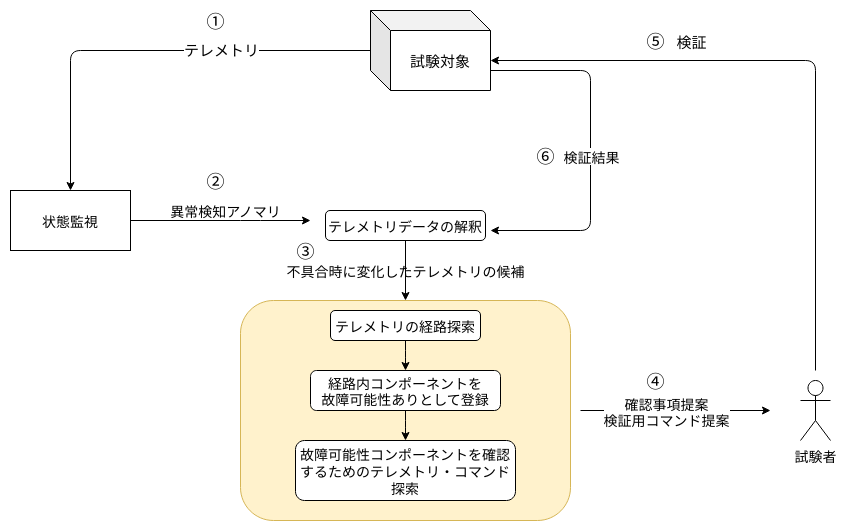
\includegraphics[height=9.0cm]{figure/fault_diagnosis_flow.png}
      \caption{不具合分析の流れ}
      \label{fig:fault_diagnosis}
\end{figure}

本手法を用いた不具合分析の流れは以下である.
\begin{enumerate}[1]
   \item 異常検知のきっかけとなったテレメトリ群を与える.
%   どこが異常値なのかを認識させる. 
   %不具合を起こしたトリガーが何なのかは分からないが,コマンドによってもたらされたかの区別だけ必要?
   \item 1で得たテレメトリに影響を与えるコマンドを送信されてから,
   地上局がテレメトリを受信するまでの一連の経路を取得する.
   \item 得られた経路内にあるコンポーネントを「故障候補」として登録する(故障仮説の生成).
   %その経路に対してコマンドパスとして入力があれば,入力の元となっているコンポーネントも故障候補に追加する.
   %ココらへんの細かい流れは図に表現できていないので,あとで説明する形を取る
   %\item 他のテレメトリを確認することによって,棄却できる「故障候補」を棄却する.
   %\item コマンドを送って得られるテレメトリ情報によって,故障候補を確認することができるコマンドの探索を行う.
   \item 打つコマンドが無くなるか,不具合原因の特定ができるまで以下を繰り返す.
   \begin{enumerate}[\textrm{4.}1]
      \item 故障候補を確認するためのテレメトリ及びコマンド探索
      \item 上で得られたコマンド及び確認事項を,人間の判断を支援する指標と共に
      提示する.
      \item システムが提示した情報を元に人が打つコマンドを選択し,仮説の検証を行う.
      \item 送信コマンドに対するテレメトリを確認し正常かどうかのフィードバックを行う.
      \item 人間からのフィードバックに応じて故障仮説の棄却及び,モデルが持つ状態の更新を行う.
   \end{enumerate}
\end{enumerate}
%
故障候補を確認するためのテレメトリ・コマンド探索の流れの詳細に関しては
後ほど言及する.

%また,本手法では故障候補は異常テレメトリが通る経路内にあるコンポーネントとしており,
%網羅的に洗い出せているとは言えない.

%実践した結果を分かりやすく表示させるように変更して,
%その結果を例に説明するのがいいかもしれない
\subsection{故障候補を切り分けるためのコマンド及び確認事項の探索}
以上で述べた不具合分析アルゴリズムにおける,
故障候補の中から切り分けを行うためのコマンド,及び
確認事項の探索に関して,本手法における仮定とともに詳細を述べる.\\
不具合が発生している状態で予期せぬ二次故障を起こさないために,
探索順序としては,衛星の状態を変えずに確認できるものを優先的に探索
することが望ましい.
%ここ表現がわかりにくい
そのため,不具合発生時に取得しているテレメトリの中から
不具合原因特定に役に立つテレメトリ情報が存在するのであれば,
そのテレメトリを確認事項として提案する.\\
その後,衛星の状態を変化させること無く
故障原因特定のために得られる情報がなくなれば,
次ステップとしてコマンドを打って得られる
情報から切り分けを行っていくことになる.
このとき,残ったコマンドで故障候補の状態を確認できるものを探索し,
上で示した指標の計算を行い提示する.
%提示するコマンド候補としては,使用するコンテキストに適した評価指標に基づいて
%上位 のコマンドを指標の値とともに提示する.
%ここにフローチャート的なものあるといいよね




%ここにモデルの説明
%これらのモデルに基づいて,実装上ではどのようなオブジェクトが生成され
%どのように関係しているのかを図示できたほうがいい
\section{事前定義モデル}
次に,以上で述べたアルゴリズムで不具合分析を行うために必要なモデル
に関して,具体的なテストケースをベースにして説明する.%言い回し

%これも既にモデル.先にどんなモデルが必要になるのかをまとめておいたほうがいいのか?
\subsection{対象とするテストケース}
今回,以下の図\ref{fig:simple_sat}の
ような簡易衛星モデルを対象にしてモデルの定義及び
不具合分析手法の実践を行う.\\
また,矢印の色が情報の方向性を表しており,赤がコマンドによる情報の伝達,
青がテレメトリによる情報の伝達である.また,矢印の種類が情報として伝わる物
を表しており,それぞれ以下のようになっている.
\begin{itemize}
   \item Signal:電気信号
   \item Power:電源
   \item Heat:熱
\end{itemize}
\begin{figure}[H]
   \centering
      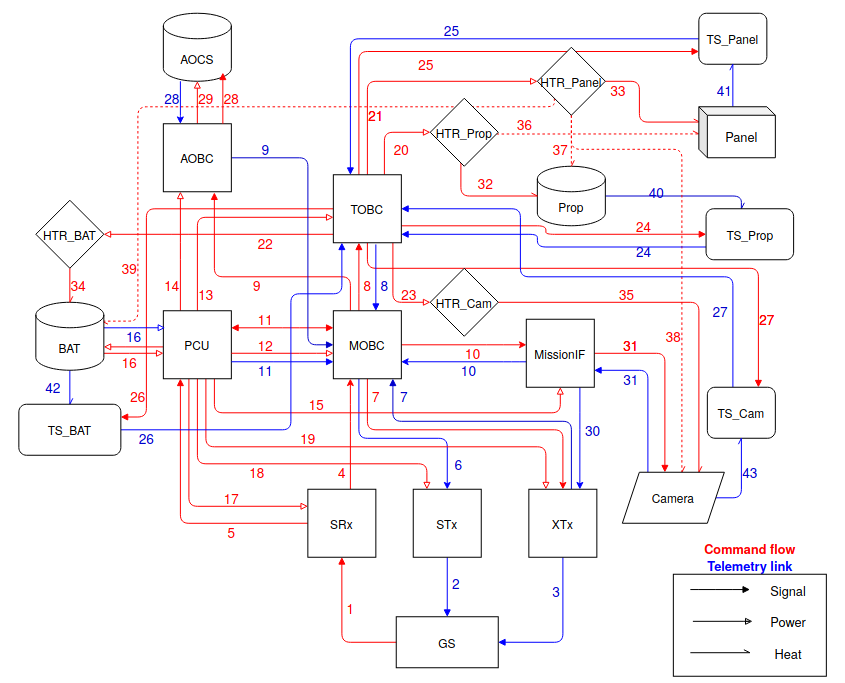
\includegraphics[height=13.0cm]{figure/satellite_diagram.PNG}
      \caption{簡易衛星モデル}
      \label{fig:simple_sat}
\end{figure}

\subsection{各コンポーネント間の接続関係モデル}
來村ら\cite{Kitamura01}は拡張デバイスオントロジーとして,
機器を構成する装置間のつながりを表現するために「ポート」と「導管」%ここの説明を考える
という概念を定義している.このオントロジーを用いて,山口ら\cite{Yamaguchi2014}
は人工衛星デバイスオントロジーを構築している.
%論文ではもう少し詳細に説明する.
これらを参考にし,以下のTable \ref{tab:link_definition}のように
接続関係を「リンク」として定義した.\\%違いを説明する必要があると思う
リンクが持つ情報としては,リンク名,接続コンポーネント,ID,伝達物,
そのリンクが正常に情報伝達を行う確率%言葉がむずい
となっており,IDが各リンク固有の識別子としてリンクを参照する際に
使用される.また,実際にコンポーネント間を接続している実態(配線やコネクタなど)を表現している
のではなく,接続関係を概念的に表現したものにすぎない.
%そのメリットは何なん?
%ほんまはちゃんとポートと導管を作ったほうが良かったんかもしれん

%\newpage
%キャプションとくっついているか確認
%図新しいのに変える
\begin{table}[H]
   \centering
   \caption{リンク定義例}
   \label{tab:link_definition}
\end{table} 
\vspace{-2zh}
\begin{figure}[H]
   \centering
      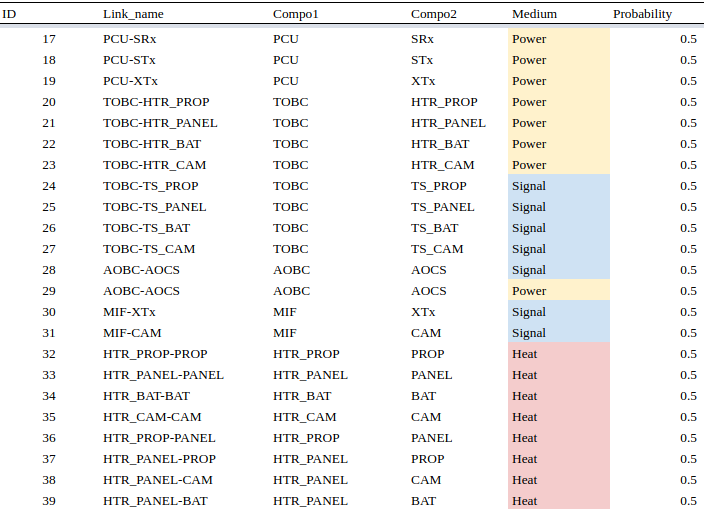
\includegraphics[height=11cm]{figure/link_definition.png}
\end{figure}

次に,コンポーネントの定義を行う.以下のTable \ref{tab:compo_link}では,
衛星システム全体で使用されている
コンポーネントのリストを作成し,各コンポーネントが接続している
コマンドリンクとテレメトリリンクを,上で定義したリンクのID
を用いて定義している.
ここで,コマンドリンクというのはコマンドによる情報の伝達で使用されるリンクであり,
テレメトリリンクというのはテレメトリによる情報の伝達で使用されるリンクである.
この時,コンポーネントが属性として持つリンクはそのコンポーネントが出力元となる場合としている.

%キャプションとくっついているか確認
%図新しいのに変える
\newpage
\begin{table}[H]
   \centering
   \caption{コンポーネント定義例}
   \label{tab:compo_link}
\end{table}
\vspace{-2zh}
\begin{figure}[H]
   \centering
      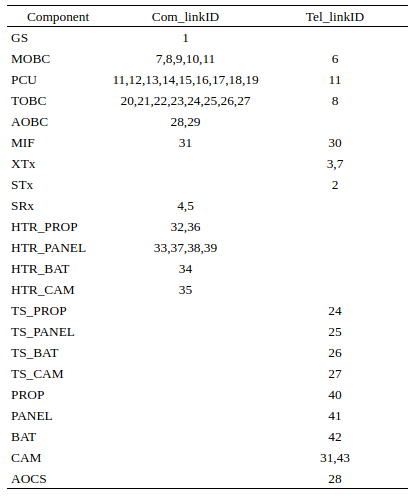
\includegraphics[width=10cm]{figure/compo_link.png}
\end{figure}

以上の情報によって,衛星内部でコンポーネント全体がどのように接続しているか
を定義することが可能になる.\\
%なんか説明が微妙
また,各コンポーネントの状態を以下の
図\ref{fig:Compo_state}のように定義する.
本研究では,簡単のため扱う状態は,各コンポーネントの電源状態,
それに伴う電力消費,姿勢変化及び,熱の発生としている.
また,電源ON/OFF状態以外にも機能を持つコンポーネントは
その機能をFunctionで定義しており,機能の
動作状態がコマンドによって操作される構成となっている.
初期状態を図\ref{fig:Compo_state}のようなファイル形式で与え,
その後の状態の更新は人間が選択したコマンドが持つ機能情報に基づいて
行うようにしている.
%現状のモデルではON/OFF状態や機能動作の正否のような2値状態のみしか扱えていないが,
%将来的にはパラメータを含む状態量も扱えるように拡張していく予定である.
\begin{figure}[H]
   \centering
      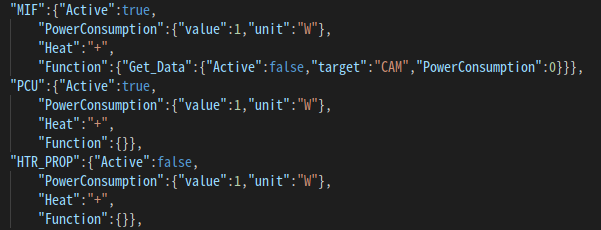
\includegraphics[height=5.0cm]{figure/Component_state.png}
      \caption{コンポーネント初期状態例}
      \label{fig:Compo_state}
\end{figure}

\subsection{コマンド・テレメトリの情報がコンポーネント間を伝わる経路のモデル}
今回の衛星モデルにおけるテレメトリ及びコマンド
を以下のTable \ref{tab:telemetry},\ref{tab:command}に定義した.\\
まず,本手法で用いるテレメトリの情報は,ID,テレメトリの名前,
テレメトリが変化するためのトリガー,テレメトリの情報が衛星内部及び地上局まで伝わる
経路である.
今回は簡単のため,状態が変化するためのトリガー(TransitionTrigger)として,
時間とコマンドのみを考えており,姿勢変化や軌道条件に依存した
状態変化は考えないことにする.また,経路は通るリンクのIDを用いて
表現している.
時間変化するテレメトリに関しては,コマンドによって状態変化をさせなくても
変化を確認することが可能なので,不具合分析の初めのアプローチに利用可能である.

%経路はjsonで記述したほうが扱いやすいし,分かりやすい.時間あれば実装も含めて修正
%経路だけじゃなくて,遷移するトリガーも加えたことを記述
%テレメトリも種別必要なんじゃね?あと,降りているかどうかという状態も必要そう.
%ここに書くかは別として
\newpage
\begin{table}[H]
   \centering
   \caption{使用テレメトリ}
   \label{tab:telemetry}
\end{table}
\vspace{-2zh}
\begin{figure}[H]
   \centering
      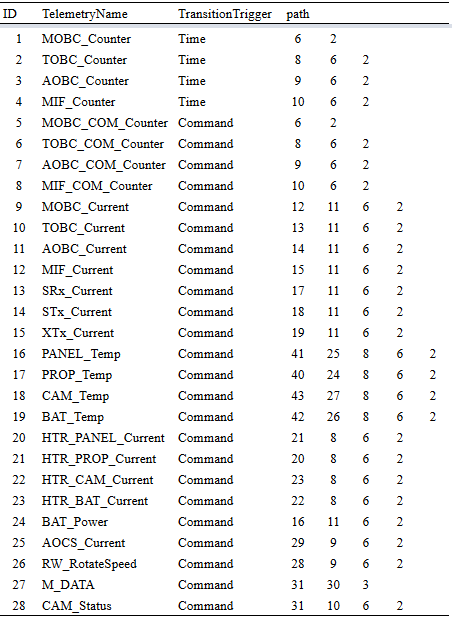
\includegraphics[width=14.0cm]{figure/TEL.png}
\end{figure}

また,コマンドの情報としてID,コマンドの名前,コマンドによって影響を受ける
テレメトリのID,コマンドの種別,コマンドによって情報が伝達する経路を与えている.
今回,Table \ref{tab:telemetry}に示すテレメトリの経路及び,Table \ref{tab:command}
に示す経路と影響テレメトリIDに関しては事前に定義したものを使用した.

また,コマンドが持つ機能によって,いくつかの種別に分類することができる.
JAXA\cite{JAXA2020}は,衛星と衛星搭載機器の機能をモデル化し,機能情報の
再利用性を高めることを目的とした手法を提案している.
今回,その手法の中の一部を採用しコマンドの種別を2種類(ACTION, GET)定義した.
また,各コマンドが持つ機能に関する情報を
以下の図\ref{fig:COM_type}のように定義している.
これによって,各コマンドが
上記で定義したコンポーネントが持つ機能を操作するという関係性を表現可能になる.
%この情報を用いて,不具合原因特定のためのコマンド
%を探索する際に有効となるコマンドを判断している.

\newpage
\begin{table}[H]
   \centering
   \caption{使用コマンド}
   \label{tab:command}
\end{table}
\vspace{-2zh}
\begin{figure}[H]
   \centering
      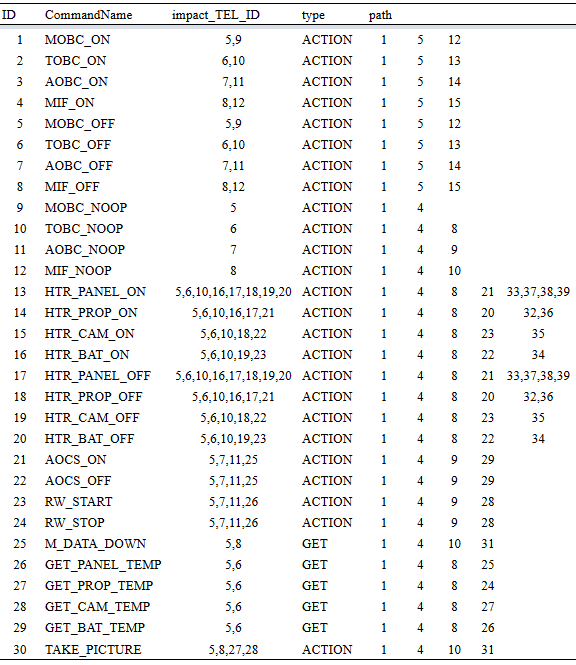
\includegraphics[width=16.5cm]{figure/COM.png}
\end{figure}

\begin{figure}[H]
   \centering
      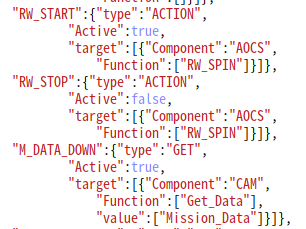
\includegraphics[height=5.0cm]{figure/COM_type.png}
      \caption{コマンドの機能モデル}
      \label{fig:COM_type}
\end{figure}


\section{コマンド評価指標}
次に,上記のアルゴリズムによって故障候補の切り分けを行う際,
人間がコマンドを選択するための指標に関して説明する.
%ここに軽く指標に関してどのような指標が必要なのか書いたほうがいいかも
不具合分析を行う際,衛星の安全を確保しながら正確な故障箇所の特定を行うことが,
地上での不具合改修に必要である.
そのため,コマンドが衛星にとって安全であることが重要である.\\
また,本研究の当初の目的は地上試験における不具合分析支援であったが,提案手法は
コマンドとテレメトリの粒度で得られる情報を用いて不具合分析を行っているため,
軌道上での運用時にも活用できると考えられる.
運用時には地上試験時とは異なり,不具合改修のための時間制約が発生することがあるため,
地上試験時とは異なる指標が必要となる.
そのため以下では,地上試験時と運用時の両方に関してコマンドを選択する上で必要な指標として
コマンドによる衛星生存性への副作用を示す指標とコマンドの故障候補の切り分け能力を示す指標
を提案し,
システムの使用状況に合わせてそれらの評価指標を切り替えることのできる
フレームワークであることを示す.

%確認することに関してはここで述べているのでこの仮定を置いていることに関してはここでいえばいいかもしれない
また本手法では簡単のため,コマンド及びテレメトリが情報を伝達する経路内に
故障候補が存在していれば,その故障候補を「確認できる可能性がある」としている.
一方で,各コンポーネントの状態を一切変えないコマンドや,コマンドを送っても
テレメトリに変化として現れない組み合わせは,不具合原因特定のために得られる情報がないため
「確認できる可能性がない」としている.\\
ここであくまでも「確認できる可能性」として記述しているのは,
情報が通る経路に故障候補が含まれていたとしても,伝達の
途中で情報が途切れてしまえば,その故障候補の状態を
確認することはできないためである.

\subsection{コマンドによる衛星生存性への副作用}
打つコマンドが安全であるかという点は,衛星の状態に依存するが,不具合発生時には
衛星の状態把握が十分に行えていない状況であるため,
網羅的にリスクを考慮した安全性を評価するのは困難である.
そこで,以下では簡単に電力と姿勢の制約を元に,コマンドの危険性を定量化する
ための指標を示す.

%BAT残量の定義がおかしいことに関して,どのような仮定をおいているのかを説明するべき
まず,運用時には発電量と各コンポーネントの電力消費状態に応じて
電力の制約が発生する.バッテリ残量が少ない状態で大きな電力を消費するコンポーネントの
電源をONにするといった行為は,衛星が生存するために必要な機能を動作させるための
電力を枯渇させる可能性があるため,危険な行為であると言える.
そのため,故障箇所の特定を行うためにコマンドを打つ際には,現在の衛星の電力状態を
把握し,コマンドを打つことで電力不足にならないかを確認しながら行動を起こさなければならない.
%もう一文くらいあってもいいかもね
コマンドを選択する際に電力に関する制約を明示的に示すことは,未熟なエンジニアが
誤ったコマンドを打つことを防ぐために効果的であると考えられる.
そのため本手法では,コマンドの副作用を示す一つの指標として「バッテリ残量」
と「コマンドを打つことによって発生する消費電力」を示すことにする.
ここでは電力による制約を簡単に表現するため,
バッテリ残量は電源がONになっている機器の消費電力のみから計算することとし,
姿勢の変化や日照条件に応じた充電量の変化は考慮していない.

次に,姿勢の制約による指標に関して述べる.
軌道上で姿勢が変化すると日照条件や入放熱量など,様々な波及効果が考えられ,
衛星の状態が大きく変化する.一方で,上で述べたように不具合発生時には
衛星の状態に不確定な要素が多く含まれているため,意図せず姿勢変化を起こし
状態を大きく変化させることは非常に危険である.
本手法で用いるモデルでは姿勢が変化することによる各状態量への影響は考慮していないが,
将来的に実ミッションで使用することを考えると,%???
姿勢変化は衛星の生存にとって
リスクの大きな動作であるとため,「姿勢変化を起こすか否か」を二つ目の指標として
提示する.

最後に,コマンドによる波及効果の大きさを示す指標に関して述べる.
上述したように,状態を大きく変化させるようなコマンドを故障個所の特定
のために用いることは望ましくない.
そこで,コマンドによって発生する衛星内部状態の変化の大きさを
%簡単にはテレメトリの数でいい気がするが..とりあえず保留
%上記で定義したコンポーネントの状態(電源状態及び機能動作状態)
%が変化した数を用いることにする.
「コマンドを打つことで変化する
テレメトリの数」を用いて定量的に示す.
これは,事前にコマンドの定義によって定められている
「コマンドに影響を受けるテレメトリ」と,人間からフィードバックを受けながら更新される
衛星内部コンポーネントの状態から求めることが可能である.この情報を示すことで,
コマンドが引き起こす衛星内部の状態変化の大きさを
人間に対して認識させることが可能である.\\
以上で述べたコマンドの副作用を示す3つの指標を以下に再掲する.
\begin{itemize}
   \item コマンドを打つ前のバッテリ残量と,コマンドを打つことによって発生する消費電力
   \item 姿勢変化を起こすか否か
   \item コマンドを打つことで変化するテレメトリの数
\end{itemize}

\subsection{コマンドの故障候補切り分け能力}
%可視時間でもいいのか?
運用時には,通信可能な時間(以下,可視時間)が限られており,その時間中に不具合原因を特定
しなければならないような時間制約がある場面が存在する.
運用形態によっては,可視時間が非可視時間に比べて非常に短いこともあり,
その際には一つの可視時間を逃すとミッション失敗につながるため,%言い方
少ないコマンド数で効率的に不具合分析が行えることが重要である.\\
%これ以下は変えたほうがいいかもしれないが,実装次第
効率的な不具合分析を行うためには,一度に確認できる故障候補の数が多いことが望ましい.
コマンドによる検証を行う際,検証結果が正常テレメトリであれば,そのコマンドとテレメトリで形成される
経路内にある故障候補は正常であると言えるため,故障候補の切り分けを行うことができる.
一方で,選択したコマンドによる検証結果が異常テレメトリであった場合,
伝達する情報が経路内のどこで異常になったかが分からなければ,その経路内に
存在する故障候補の切り分けを行うことはできない.
そのため,経路内に多くの故障候補が存在する場合でも,
切り分けの能力が高いとは言えない.故障候補の切り分け能力を考えるためには,
検証結果が正常,異常に関係なく経路内にある
故障候補をどれだけ確認できるかが重要になる.
以下では,故障候補にあるリンクが正常に情報を伝達できる確率を用いて,
コマンドが確認できるリンクの数を見積もる.

%あとここで言っている正常はつながりが切れていないかという点であることを説明する?
各コマンドによって情報が伝達し,テレメトリとして地上局に返ってくる経路によって,
確認する対象のリンクまでに通る経路が異なる.
その各経路に存在するコンポーネントをつなぐリンクが正常である確率を
$P(l = \text{normal})$,異常である確率を$P(l = \text{abnormal})$ %確率Pも斜体じゃないほうがええかも
として与える.
あるリンク$l_i$を確認するためには,リンク$l_i$が接続されているコンポーネントまでの経路
が正常であることが必要である.このことから,「リンク$l_i$を確認することができる確率」
がそれぞれの経路によって定まる.このことを以下の図\ref{fig:route}に示す例を用いて示す.
以下では簡単のため,$P(l_i = \text{normal}) = P(l_i = \text{abnormal}) = 0.5$であるとし,
太矢印になっている箇所が故障候補である.また故障候補以外は正常であるとし,
正常なリンクに関しては$P(l_i = \text{normal}) =1$である.\\
\begin{figure}[H]
   \centering
      \begin{tabular}{c}
         \begin{minipage}{0.30\hsize}
         \centering
         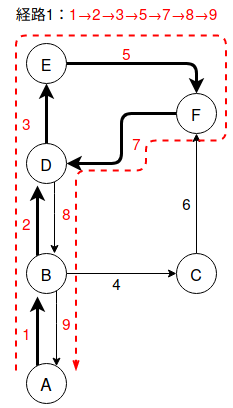
\includegraphics[height=7cm]{figure/route1.png}
          %  \caption{}
            \label{fig:route1}
         \end{minipage}
         \begin{minipage}{0.30\hsize}
         \centering
         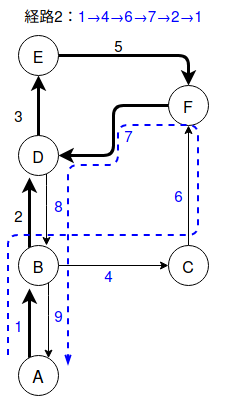
\includegraphics[height=7cm]{figure/route2.png}
         %\caption{}
            \label{fig:route2}
         \end{minipage}
         \begin{minipage}{0.30\hsize}
            \centering
            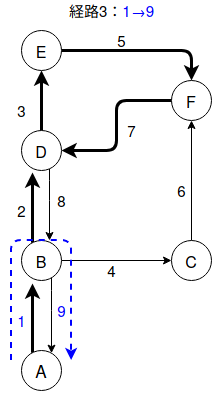
\includegraphics[height=7cm]{figure/route3.png}
            %\caption{}
               \label{fig:route2}
            \end{minipage}
      \end{tabular} 
      \caption{故障候補とそれを確認するための情報伝達経路の例}%ここも変えたほうがいいかも
      \label{fig:route}
\end{figure}
図\ref{fig:route}では,あるコマンドC$_1$によって影響を受けるテレメトリ
が3つ存在する場合を示している.
各テレメトリとコマンドC$_1$が形成する経路は異なり,それぞれ経路1,2,3としている.\\
この時,それぞれの経路に関して
リンク1を確認することができる確率を考えることにする.まず,経路1でリンク1の確認をするためには
ノードBからノードDまでの経路(2,3,5,7)
が正常である必要がある.%正常の定義を明確に
ここで,経路を表す記号をR,経路内にある故障候補リンクの集合を$\mathbb{F}$とすると,
経路1を通る情報でリンク$1$を確認することができる確率は
\begin{eqnarray}
   P(l_{1} | \text{R}_1) &=& \prod_{i\in\mathbb{F}_1,i\neq 1} P(l_{i} = \text{normal})\\
     &=& \left( \frac{1}{2}\right)^4
\end{eqnarray}
であることが分かる.ここで,R$_1$は経路1,また
\begin{eqnarray}
   \mathbb{F}_1  &=& \{ 2,3,5,7\} 
\end{eqnarray}
である.\\
同様に経路2,3に関してもリンク$1$を確認することができる確率を求めると
\begin{eqnarray}
   P(l_{1} | \text{R}_2)  &=& \prod_{i\in\mathbb{F}_2,i\neq 1} P(l_{i} = \text{normal})\\
   &=& \frac{1}{2}\\
   P(l_{1} | \text{R}_3)  &=& \prod_{i\in\mathbb{F}_3,i\neq 1} P(l_{i} = \text{normal})\\
   &=& 1
\end{eqnarray}
となる.
このように,あるリンク$l_i$を通る経路が複数存在する場合,
経路に依存してそのリンク$l_i$を確認できる確率(以下では確認可能性とする)が変わる.
%なんで最大値を取るようにするのかの説明が必要になるかもしれない
ここで,あるコマンドC$_k$による情報伝達経路の中で,リンク$l_i$を通る経路
が複数存在する場合には,リンク$l_i$に対する確認可能性が最大となる
経路を用いて確認すればいいので,コマンドC$_k$による
リンク$l_i$の確認可能性はそれらうちの最大値を取るものとする.
コマンドC$_k$が影響を与える各テレメトリと成す経路の内,リンク$l_i$を含むものを
$\mathbb{R}_{ki} = \{ \text{R}_{1_i}, \cdots ,\text{R}_{N_{ki}} \}$(ただし$N_{ki}$は
リンク$l_i$を含む経路の数)とすると,
コマンドC$_k$によるリンク$l_i$の確認可能性は
\begin{eqnarray}
   P(l_i|\text{C}_k) &=& \max  \{ P(l_i|\text{R}_{1_i}), \cdots ,P(l_i|\text{R}_{N_{ki}}) \}
   \label{eq:P li Ck}
\end{eqnarray}
となる.\\
式(\ref{eq:P li Ck})は経路$\mathbb{R}_{ki}$内にある故障可能性リンク
全てに対して求めることができるので,
これらの平均を取り,そのコマンドの「平均確認可能性」と定義する.
平均確認可能性は,コマンドC$_k$が影響を与える各テレメトリと成す経路を
$\mathbb{R}_{k} = \{ \text{R}_{1}, \cdots ,\text{R}_{N_{k}} \}$とし,
それらに含まれる故障可能性リンクの数を$N_{F_k}$とすると
\begin{eqnarray}
   P_m(\text{C}_k) &=& \frac{1}{N_{F_k}}\sum_{i=1}^{N_{F_k}}P(l_i|\text{C}_k)
\end{eqnarray} %記号何がええんやろ
と表すことができる.平均確認可能性は,コマンドとテレメトリが通る経路に含まれる
故障候補のうち,どれだけのリンクの状態を確認できるかという指標である.
つまり,この指標が高いほど経路内に存在する故障可能性リンクの多くを
確認できるということになる.%これいらんかも
%それ以下でもそれ以上でもないのか??

また,平均確認可能性を経路$\mathbb{R}_{ki}$内にある故障可能性リンクの数$N_{F_k}$
にかけると,コマンドC$_k$によって確認できるリンク数の期待値を求めることができ,
\begin{eqnarray}
   E(\text{C}_k) &=& N_{F_k}P_m(\text{C}_k)\\
   &=& \sum_{i=1}^{N_{F_k}}P(l_i|\text{C}_k)
\end{eqnarray} 
となる.これを「確認可能リンク数」と定義する.

ここで,図\ref{fig:route}に示すコマンド1に関して平均確認可能性及び,
確認可能リンク数を計算してみると
\begin{eqnarray}
   P_m(\text{C}_1) &=& \frac{1}{N_{F_1}} \{P(l_{1} | \text{C}_1) + P(l_{2} | \text{C}_1) +P(l_{3} | \text{C}_1)
   +P(l_{5} | \text{C}_1) + P(l_{7} | \text{C}_1)\} \\
   &=& \frac{1}{5} \{ 1 + \frac{1}{2} + \left( \frac{1}{2}\right)^4 + \left( \frac{1}{2}\right)^4
    + \left( \frac{1}{2}\right)^4 \}\\
    &=& 0.3375 \\
   E(\text{C}_1)  &=& 1.6875
\end{eqnarray} 
となる.
結果からわかるように,通る経路に存在する故障候補の数
が必ずしも確認できるリンクの数に対応しているわけではない.
故障候補にあるリンクを通ることで不確定性が蓄積されるため,全体として経路内にある
リンクを確認できる確率は小さくなる.
平均確認可能性が高く,確認可能リンク数も高いものが
故障候補の切り分け能力が高いコマンドであると言える.

リンクの正常確率をもとにすると,ある経路を通るテレメトリが正常もしくは
異常となる確率を算出することが可能になる.そのため,あるコマンドを選択した際に
影響を受けるテレメトリに対して,検証結果を

全体としていくつのコマンドが必要になりうるのかを算出する.


以上では簡単のため,各リンクの正常確率は0.5として統一していたが,
事前にモデルに組み込むことが可能であるため,実際の衛星に適した正常確率を考える
ことで,より効率的に故障個所の特定ができると考えられる.
%ここの説明微妙すぎるから修正
例えば,衛星の主要通信ラインである受信機と地上局間のリンクや,OBC間の
リンクは信頼性が高いと考え,正常確率を高く設定したり,
新規実装項目に関しては検証が足りていない可能性があるので,低い正常確率
を設定したりするなど,人間の判断でモデルに工夫を加えることが可能である.


%こんなんできていないので今後の課題として提示するにとどめる.
また,これらの信頼性を試験結果から学習させることによって,対象とする衛星に対する
モデルの再限度を高め,効率的な不具合分析を行うことが可能になる.

\begin{comment}
   
このことを踏まえて,あるコマンドとテレメトリのペアによって形成される経路(R)を通る情報によって
故障候補の確認を行う際,経路内に含まれる故障候補の数($N_F$とする)と
確認できるリンクの数の期待値($E$(R))の割合が,その経路を作るコマンドとテレメトリのペアが,
経路内の故障候補の内どれだけ確認することができるかを示している.\\
故障可能性リンクが多く含まれた,不確定性の大きな経路を通ると,

上で述べたように,切り分けを行っていくためには確実性が重要である.%???
そのため,その経路の「正の効果」を示す指標の一つとして確実性($C$(R)とする)を以下のように定義する.
\begin{eqnarray}
   C(\text{R})  &=& \frac{E(\text{R})}{N_F}
\end{eqnarray}
%ここらへん実装まで終わらして,ちゃんと有効であることを示せないと伝わらなさそう.
%有効でなければやり直しやが..

以上では,コマンドとそれによって影響を受けるテレメトリとのペアによって形成される経路に対して
「正の効果」を定義していたが,各コマンドが影響を与えるテレメトリは複数存在することが多くある.
人間が選択する際にはコマンドに対して指標が必要である.\\
あるコマンドに関連する経路が複数ある場合,それらに関する「確認可能リンク数」及び「確実性」
の単純和を取るだけでは対象としているリンクに被りが生じるため,コマンドの効果を表している
とは言えない.
そこで,各経路で被りが生じているリンクに関しては,
そのリンクを通る経路の中で距離が最短な経路が確認を行うものとし上の指標を再定義を行う.
あるコマンド(C$_k$とする)が影響を与える各テレメトリと成す経路の集合を
$\mathbb{R}_k = \{ \text{R}_{1}, \cdots ,\text{R}_{N_k} \}$(ただし$N_k$はコマンドC$_k$
によって形成される経路の数)とする.
%これは実装で必要になるかも
%また$\mathbb{R}_k$は経路長さの昇順でソートされている
また,各経路(R)$_{i}$に含まれる故障候補
の集合$\mathbb{F}_{i}$の直和を取り%少し間違っているから修正
$\mathbb{R}_k$に含まれる故障候補の集合を,
%なんかいい方法思いつかんから保留
\begin{eqnarray}
    \mathbf{F_k} &=& \sum_{i=1}^{N_k} \mathbb{F}_i
%    \bigcup_{i=1}^N \left( \bigcup_{i=1}^N \mathbb{F}_i - \bigcap_{i=1}^N\right) 
\end{eqnarray}
とし,$\mathbf{F_k}$に含まれるリンクの数を$\mathbf{N_{F_k}}$とする.
この時,C$_k$の「確認可能リンク数」及び「確実性」は以下のようになる.
\begin{eqnarray}
   E(\text{C}_k)  &=&\sum_{i\in \mathbf{F_k}} \prod_{j\in \mathbf{F_k}, j\neq i} P(l_i=\text{normal})  \\
   C(\text{C}_k)  &=& \frac{E(\text{C}_k)}{\mathbf{N_{F_k}}}
\end{eqnarray}
\end{comment}

%ここに情報量を組み込むといいかも?めんどくさい

%ここ洗練させる
\subsection{評価指標の使い分け}
次に,地上試験と軌道上での運用とで上述した指標の使い分けに関して
説明する.
\begin{comment}
   
%エントロピー使うなら平均は取らない.
まず,コマンドを打つことによってどれだけの情報が得られるかという点から,
そのコマンドを打つことによる情報量を考えた.

その指標として,コマンドの能力を情報量(エントロピー)の定義から考えた.
無理にエントロピーを使うのは間違っている気がする.情報量という考え方が妥当ではないか?
確率分布になっていないことを考えると.

コマンド$j$による切り分けの効果の指標を以下に定義する.\\
コマンド$j$が確認できるリンクの集合を$\mathbb{L}_j$とする.
この時,集合に含まれるリンクは$l_i\in \mathbb{L}_j$とする.
また,
「$\mathbb{L}_j$を確認する」という事象を$\Omega$とすると,
各リンク$l_i$を確認するという事象$E_i \in \Omega$として,

ここで,各リンクの状態を確認する方法として,本手法ではコマンドによるアクセスのみを考えているので
「リンク$l_i$を確認する」という事象と,「リンク$l_i$を確認できるコマンドを選択する」
という事象の確率は等価である.%各コマンドを選ぶ確率は等しいという仮定が入っているような気がする.
よって,「リンク$l_i$を確認する」という事象の確率は式(\ref{eq:Pi})
で与えられる.この時,事象($E_i$)が起こった時に受け取る(選択)情報量$I_i$は式(\ref{eq:I_i})
で定義される.

\begin{eqnarray}
   P(E_i) &=& \frac{\text{Number of command which can verify Link }i}{\text{All command number}} \label{eq:Pi}\\
   I(E_i) &=& -\log{P_{i}} \label{eq:I_i} \\
\end{eqnarray}
確率$P(E_i)$は確率分布であるという説明が必要

よって事象$\Omega$による平均情報量は
\begin{eqnarray}
   H(P) &=& -\sum_{E_i \in \Omega} P(E_i)\log{P(E_i)} 
\end{eqnarray}
となる.定性的な意味としては,コマンドを打つことによってどれだけの情報
が得られる可能性があるかを示している.

コマンドが絞り込むことのできる能力という点はどうする?

以上の指標を踏まえた上でどのように提示し人間の判断を支援するのかを考える.
\end{comment}

%地上試験と運用時の両方で使い分けることのできるフレームワークであることを示す.
地上試験では,電源供給に関してはバッテリではなく安定化電源を用いた試験コンフィギュレーションで
行うことが多い.そのため,上述した電力の制約に関しては地上試験で考慮する必要はない.
また,試験時は衛星を試験台に固定して行うため,姿勢変化に関する制約も考慮する必要は
ないと考えられる.
これらを踏まえると,地上試験で安全を重視して二次故障などを引き起こさないように
切り分けを行うためには,波及効果の大きさを示す指標である
「コマンドによって影響を受けるテレメトリの数」が小さなコマンドを選択すれば良い.\\
また,地上試験では衛星全体ではなく部分的なコンポーネントを組み上げた状態による試験も多数行う.
システムを構成するコンポーネントの種類によっては,コマンドの効果によって
二次故障が発生する可能性は低い場合も考えられる.
そのような際には,「平均確認可能性」及び「確認可能リンク数」
が大きなコマンドを選択することで効率的な切り分けが行える.

%地上試験での具体例を挙げて,指標の中で何を重視すればいいのかという説明をする
%確実性の必要性がよくわからないという指摘.これが高いと,コマンドが持つ能力の
%分を確認できる.つまり不確定な領域をなるべく通らすに故障候補を確認できるということ

一方で,運用中は上述した電力や姿勢に関する制約を考える必要がある.また,
可視時間中に不具合原因の特定を行わなければならないなどの
時間制約の厳しい条件下での分析が必要になることもある.
そのような時には,リスクを大きく取りつつ効果の大きなコマンドを選択する必要がある.
よって,運用時は上で示した全ての指標を元に,リスクと効率のトレードオフを考えながら
コマンドの選択を行う必要がある.

\expandafter\ifx\csname ifdraft\endcsname\relax
  \end{document}
\fi
\expandafter\ifx\csname ifdraft\endcsname\relax
\documentclass[11pt]{jsreport}
\usepackage{mypackage}
\begin{document}
\fi

\chapter{本手法による不具合分析の実践と評価}

\section{概要}
本性では,提案手法を用いた不具合分析の具体的な流れをみるために,
いくつかの事例を取り上げて実践した結果を示す.
以下では,まず実際に故障箇所特定が行えた事例を取り上げる.
その結果に関して,コマンドを選択する際に優先する指標によって検証プロセスが異なること
を述べ,評価指標に関する考察を行う.また,その例に対して
所属する研究室の方々に実践頂いた結果との比較に関しても示している.\\
次に,本手法のみでは故障箇所の特定を上手くできなかった事例を取り上げ,
そこから得られた知見に関して述べる.\\
%ここら辺もう少し見るところがある気がする.
%ここはどうするかなあああ
最後に,本手法によって扱うことのできる故障の種類に関する限界を述べ,発展させるために必要な
方針に関して議論を行う.

\newpage
\section{実践例}
\subsection{故障箇所の特定ができた例(ヒータの接触不良)}
まず,以下の図\ref{fig:fault_mode1}のような故障を考え,
不具合分析を行っていく.\\
%図の配置を考える.
\begin{figure}[H]
   \centering
      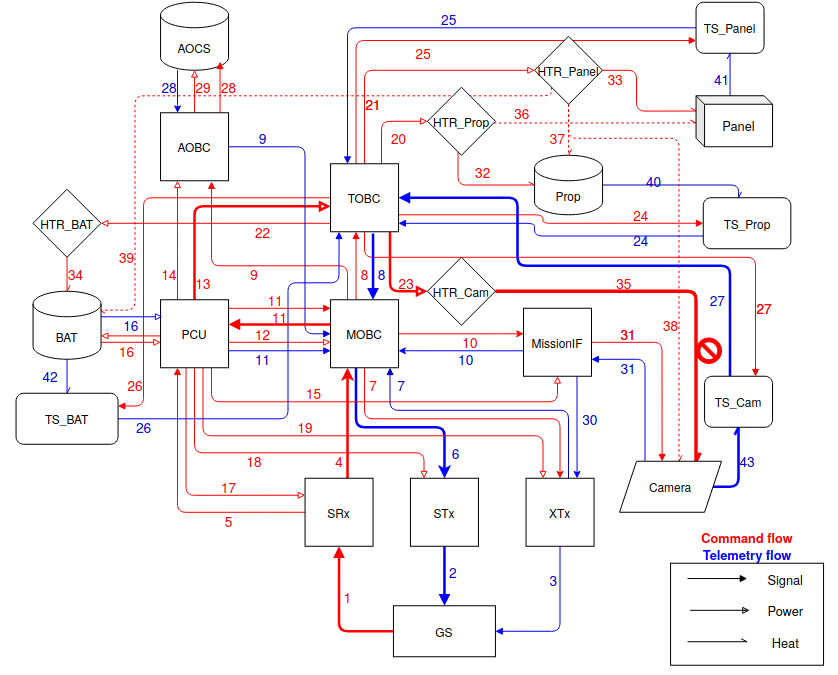
\includegraphics[height=13.0cm]{figure/fault_mode1.png}
      \caption{故障箇所:リンク32(推進系ヒータ−推進系間)の時の故障候補}
      \label{fig:fault_mode1}
\end{figure}

%問題設定の与え方として,各コンポーネントの状態はどのようになっているかを示したほうが良くないか?
%Methodologyの中で言及できているのか要確認
図\ref{fig:fault_mode1}に示すような
推進系ヒータ‐推進系間でのヒータ接触不良が発生している場合を考える.
この時,異常検知の際の不具合事象としては,
\begin{itemize}
   \item 推進系ヒータONコマンド(ID:14)を送信したのに,推進系温度(ID:17)が上昇しない
\end{itemize}
という事象である.\\
%つまりは正常モデルを元に考えているからこうなる
ここで,本手法では前章で述べたように衛星内部コンポーネントの初期状態として,
送信したコマンドによってもたらされる状態変化が起こっているものとして与えている.
そのため,不具合事象の際に送っているコマンド「推進系ヒータON」によって,
推進系ヒータは電源ON状態であると仮定し,以下の検証用コマンドの探索を行っている
ことを述べておく.
%これ実は別にどっちの状態にしてても,検証はできるんやけどな..
%ほんまは不具合検知コマンドとテレメトリのペアを除外する必要はないんかもな...

以下に,この事象に本手法を適用した例を示す.
まず,図\ref{fig:tel_phase},\ref{fig:TEL_process}に
故障候補の決定及び,テレメトリ情報を用いた確認の段階に関して
コンソールへの出力結果と切り分けの流れを可視化したものを示す.
故障候補の決定では,不具合事象を検知するきっかけとなったコマンドとテレメトリが形成する
経路を探索し,targetTEL,targetCOMとして提示している.\\
その後,時間変化するテレメトリ情報を用いて確認できる故障候補を提示し,
返ってくるテレメトリが正常(OK)か否(NG)かを入力させることで,切り分けを行っている.

\begin{figure}[H]
   \centering
      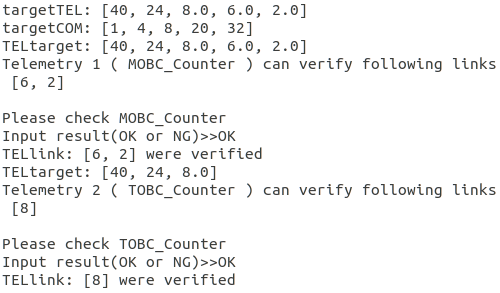
\includegraphics[height=5.0cm]{figure/COM14_TEL17_TEL_phase.png}
      \caption{テレメトリによる確認}
      \label{fig:tel_phase}
\end{figure}
\begin{figure}[H]
   \centering
      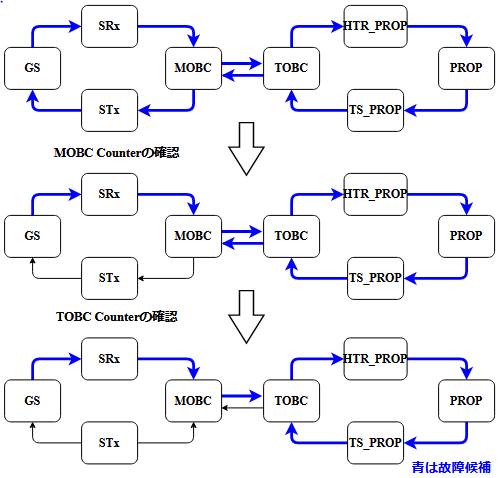
\includegraphics[height=7.5cm]{figure/TEL_process_HTR_PROP_fault.png}
      \caption{テレメトリの確認による故障候補切り分けの流れ}
      \label{fig:TEL_process}
\end{figure}

%もう少し説明が必要そう
\begin{figure}[H]
   \centering
      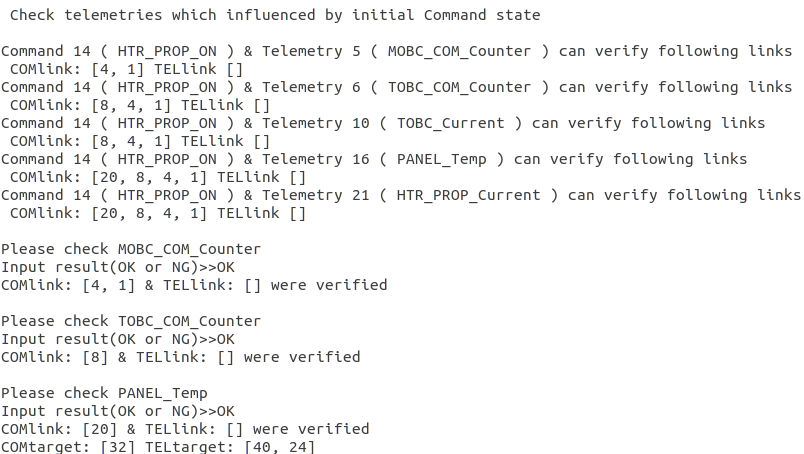
\includegraphics[height=7.0cm]{figure/COM14_TEL17_iniCOM_phase.png}
      \caption{初期コマンドによる情報を用いた確認}
      \label{fig:ini_COM_phase}
\end{figure}
\begin{figure}[H]
   \centering
      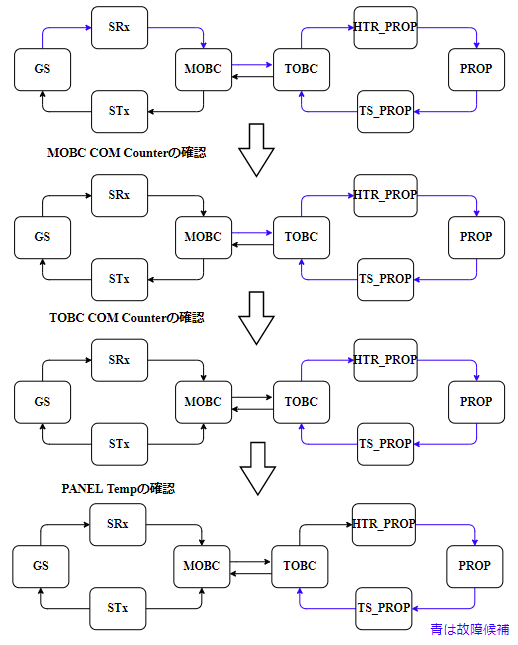
\includegraphics[height=10.5cm]{figure/iniCOM_process_HTR_PROP_fault.png}
      \caption{初期コマンドに影響を受けるテレメトリの確認による故障候補切り分けの流れ}
      \label{fig:iniCOM_process}
\end{figure}

\newpage
次に,図\ref{fig:ini_COM_phase}及び図\ref{fig:iniCOM_process}に示すのが,
不具合発生時に送信していたコマンド情報から
考えられるテレメトリの変化を用いて故障候補の確認を行う段階である.
今回は,初期コマンドとしては異常検知の際に送ったコマンド(推進系ヒータON)のみ
を考えている.
確認可能性の高い経路を形成するテレメトリから順に表示され,人間に確認をさせているのが分かる.

最後に,以下の図\ref{fig:COM_candidate}に示すのが,上記の流れを経て残った
故障候補を確認できるコマンドを探索し,指標と共に提示した結果である.
残った故障候補は,
\begin{itemize}
   \item コマンドリンク32:推進系ヒータ‐推進系間
   \item テレメトリリンク40:推進系‐推進系温度計間
   \item テレメトリリンク24:推進系温度計‐TOBC間   
\end{itemize}
である.
この時,探索結果として表示されたのはコマンド13(パネルヒータON)と18(推進系ヒータOFF)
であり,これらのコマンドに関する指標が図\ref{fig:COM_candidate}のように示されている.\\
図中においてPm(C)が「平均確認可能性」,E(C)が「確認可能リンク数」,
N(C)が「検証コマンド総数」を表している.
またコマンドの衛星生存性への副作用を示す指標に関しては,
Remain Powerが「コマンド送信前のバッテリ残量」,Power Consume
「コマンド送信による消費電力」,
Impacted TEL numが「コマンドによって影響を受けるテレメトリの数」,
Attitudeが「姿勢変化を起こすか否か」を示している.
Attitudeに関しては,姿勢変化を起こす場合は「Change」,起こさない場合は
「Keep」と表示するようにしている.

\begin{figure}[H]
   \centering
      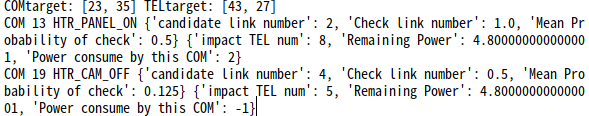
\includegraphics[width=15.0cm]{figure/COM_candidate.png}
      \caption{コマンドの選択肢表示及び検証過程}
      \label{fig:COM_candidate}
\end{figure}
以下の図\ref{fig:COM_process_HTR_fault}に,探索されたコマンドに関して各コマンドを選択し
検証を行ったプロセスを示す.
どちらのコマンドから開始しても最終的に,今回想定した故障箇所である「推進系ヒータ−推進系間(リンクID:32)」
が故障箇所であると特定された.

\begin{figure}[H]
   \centering
      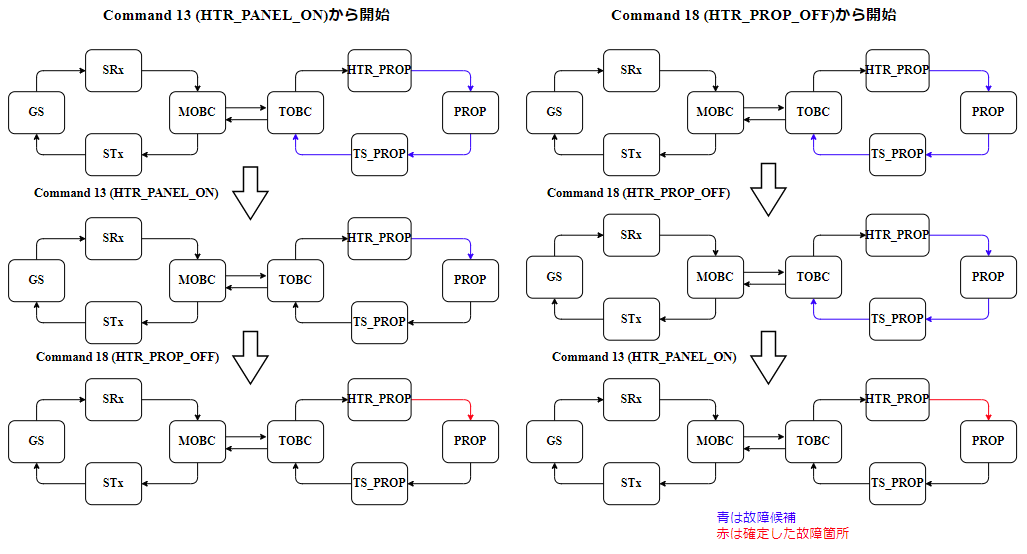
\includegraphics[height=8.0cm]{figure/COM_process_HTR_PROP_fault.png}
      \caption{ヒータ接触不良時の各検証プロセスの流れ}
      \label{fig:COM_process_HTR_fault}
\end{figure}


\subsection{コマンドの故障候補切り分け能力を示す指標に関する考察}
%ここの文言も微妙
上で示した例(ヒータ接触不良)に関して,コマンドを選択する際に優先する評価指標によって
図\ref{fig:COM_process_HTR_fault}のように検証プロセスの違いが生じた.
この結果の違いに基づき,提示された評価指標が持つ意味を考察する.

図\ref{fig:COM_candidate}にあるように提示された2つのコマンドを比較すると,
「平均確認可能性」はパネルヒータONコマンド(13:HTR\_PANEL\_ON)が高く,
「検証コマンド総数」は推進系ヒータOFFコマンド(18:HTR\_PROP\_OFF)が小さくなっている.
パネルヒータONコマンドから検証を開始した場合,初めに
「推進系−推進系温度計間(テレメトリリンク40)」,「推進系温度計−TOBC間(テレメトリリンク24)」
の正常が確認できており,
1つのコマンドによる確認で故障候補が1つのリンクにまで絞り込めている.
最終的に,推進系ヒータOFFコマンドを送信した際に%何のテレメトリで??
推進系温度の変化が見られなかったことから「推進系−推進系温度計間(テレメトリリンク32)」
の異常が確認でき,故障箇所を特定している.\\
一方で,推進系ヒータOFFコマンドから検証を開始した場合,
1つ目の検証では推進系温度に変化が見られず,状態変化を確認できないため,
故障候補の切り分けをすることができない.一方で,故障候補の中に
確実に故障箇所が存在することを確かめることができる.
次に,2つ目のコマンド「パネルヒータON」で推進系温度の上昇を見ることができるため,
先程のプロセスと同様の切り分けができ,故障箇所の特定ができている.

運用時,通信が不安定であり不具合分析に使える時間が明確でない時には
一度のコマンドで多くの確認ができることが望ましい.
そのため,図\ref{fig:COM_candidate}において「パネルヒータON」コマンドから送信する
検証プロセスが良いと言える.
これを元に考えると,
平均確認可能性が高いコマンドから送ると,一回のコマンドで多くの絞り込みが行える可能性が高いと言える.
より厳しい時間制約の際には,最後まで検証作業を行うことができるという保証はない.
そのため,平均確認可能性が高いコマンドを優先的に選択して各コマンドによって得られる切り分けの効果を
大きくすることが望ましい.

一方で検証コマンド総数が小さなコマンドを優先的に選択した場合,
少ないコマンド数で絞り込みを行える可能性があるが,
この指標はあくまで,故障箇所を特定するまで検証を行うことを前提としてコマンドの数を計算している.
そのため,故障状態によっては
見積もられた数以上のコマンドを送信する必要があり,時間制約が厳しいときには十分に
絞り込みを行えないまま検証作業を終えることになる.
このことを踏まえると,検証コマンド総数は不具合分析を最後まで行うことができる保証がある時に,
優先的に考えることで,全体で打つコマンドの数を少なくできる可能性があると言える.

%複数故障を考えた場合,指標の選択基準によって
%探索プロセスが変化する.

\subsection{本手法と人間の不具合不具合分析の違い}
上で示した不具合事象「推進系ヒータONコマンドを送った時,推進系温度が変化しない」
に関して,想定した故障状態に関する情報を与えずに
不具合分析を行う際の過程(送信するコマンド,コマンドを選択する理由,
確認するテレメトリ)を不具合分析の経験が豊富な本研究室の先輩方に伺った.\\
与えた情報としては,以下に示す通りであり,コマンドやテレメトリが通る経路や,
コマンドが影響を及ぼすテレメトリに関する情報は与えなかった.
\begin{itemize}
   \item 衛星システムのコンポーネントの接続関係図
   \item システムを構成するコンポーネント及びその電源状態
   \item コマンド及びテレメトリの定義情報(何の機能を持つコマンドなのか,テレメトリに含まれる情報)
\end{itemize}
質問内容は以下であり,コマンドによる不具合分析を始める段階からの意思決定を対象にしている.
\begin{itemize}
   \item 不具合分析を開始する際に初めに送信するコマンドとその理由
   \item 初回の検証で何のテレメトリ情報を確認するか
   \item 上で送信した結果が正常もしくは異常であった場合に次に選択するコマンド及びその理由
   \item 2回目の検証で何のテレメトリ情報を確認するか
\end{itemize}
以下の図\ref{fig:first_selection}に,初回の検証で選択するコマンドの調査結果
を示す.本手法で検証用コマンドとして提案された2つのコマンド「推進系ヒータOFF(HTR\_PROP\_OFF)」と
「パネルヒータON(HTR\_PANEL\_ON)」を選択している人が半数以上を占めていることから,今回の問題設定では
本手法による検証用コマンドの探索は人間の推論に近いと言える.
また,提示された選択肢以外のコマンドを選択する人が一定数いたが,これらを選択した理由を見ると,
これらのコマンドによって回答者が確認しようとしている事項は既に確認しているとして問題を設定していたため,
問題での前提条件に対する認識の違いによるものであった.また,それらの回答者に関しても
2回目のコマンド選択では,「パネルヒータON」を選択しており,検証用コマンドとして本手法による探索と
同じような推論を行っていると言える.

\begin{figure}[H]
   \centering
      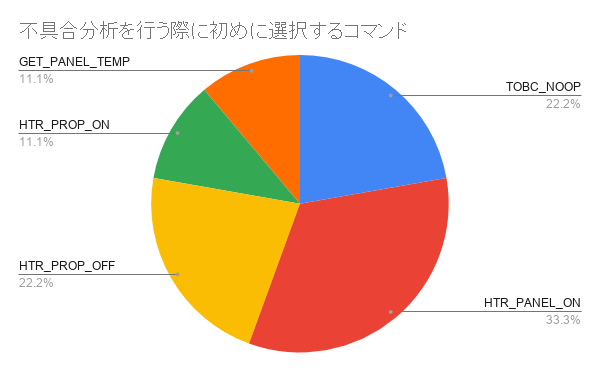
\includegraphics[height=6.0cm]{figure/first_selection.png}
      \caption{不具合分析時に初めに選択するコマンドの調査結果}
      \label{fig:first_selection}
\end{figure}
また,このコマンドを選択した理由を見ると,「パネルヒータON」コマンドを送る人は
積極的に故障候補の絞り込みを行う目的で選択しており,「推進系ヒータOFF」コマンドを送る人は,
故障していると考えられる推進系ヒータに通電を続けるのが危険であると考え,安全を考慮して
このコマンドを選択していた.
本手法でコマンドの安全性を示す指標として提示するものは,電力と姿勢による制約からくるものと,
状態をどれだけ変化させるかという点から提案を行っていた.
しかし,不具合発生時に故障箇所が含まれている可能性があることを考えると,
そのままの状態を保持することが危険であるという考え方もできる.
そのため,安全状態に戻すという視点での指標の提案が必要であると考えている.\\
また,状態を不具合発生前の状態に戻すコマンド「推進系ヒータOFF」は同時に,
故障候補を検証可能なコマンドであることが分かる.人間による不具合分析では
このことを意識せずに,故障候補切り分けのための情報を見逃してしまうことも多い.
本手法を用いることで,このコマンドも検証用コマンドとして提示することで切り分けのために必要な情報を
見逃すことを防ぐことにつながる.

次に,初回の検証結果が異常であった場合に次に選択するコマンドに関して以下の図\ref{fig:second_selection}
に調査結果を示す.初回に選択するコマンドが本手法で提案したものと一致していたのに対し,
次に選択するコマンドは大きなばらつきが見られた.
こちらに関しても,これらのコマンドを選択した理由を見ると,故障候補の特定よりも
二次故障の発生を防ぐために安全を考慮してコマンドを選択した場合や,
故障候補をより網羅的に洗い出したことによる検証プロセスの違いであることがわかった.\\
前者に関しては,上述したように不具合状態を保持することによる危険を考えており,
本手法では扱うことができていない概念である.\\
また後者に関しては,本手法では故障候補の洗い出しは不具合発生時のコマンドと
テレメトリが通る経路のみに限定しているが,不具合分析経験が豊富な人による推論では,
コマンドによる状態変化を起こすための電力供給源を考えた場合や,コンポーネントの機能単位
の回路の故障を疑ったものが見られた.実際の不具合発生時では,このようにコンポーネント間の
接続関係だけでない機能間のつながりや,状態変化によって発生する波及効果によって
他のコンポーネントに影響を与えることも考えられるため,今後の課題としてより網羅的な故障仮説の生成
に取り組む必要があると考えている.\\%ここ違う気がする.言いたいのはこれじゃない

\begin{figure}[H]
   \centering
      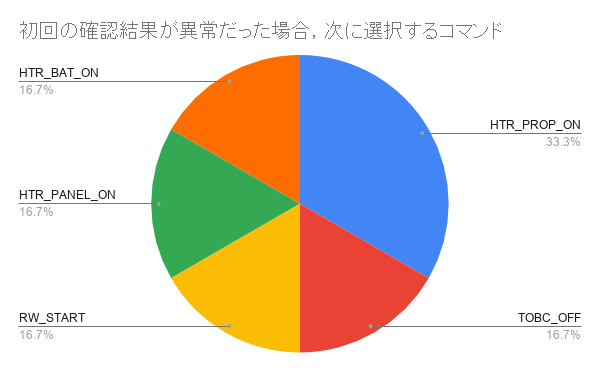
\includegraphics[height=6.0cm]{figure/second_selection.png}
      \caption{初回の検証で確認したテレメトリが異常であった場合}
      \label{fig:second_selection}
\end{figure}

また,本手法による故障箇所特定は単一故障を前提としたアルゴリズムとなっていたが,
複数故障を考慮した分析を行う人も見られた.その場合,安全なコマンドを評価する
ためには全ての故障候補の組み合わせの場合の数だけコマンドによる影響を考慮する必要がある.
それらの組み合わせに対して波及効果までを考え,安全性を評価できるのは人間の強みであると言える.
一方で,このように多くの候補を考えることは多くの知識と経験を要する作業である.
経験の少ない人物が安全性の評価を十分に行うことを支援するために,複数故障を考慮した
検証作業に関しても考慮する必要があることが分かった.
%ここも微妙やな!

%最後に違いをまとめる?
%以上のように,本手法を用いた不具合分析と人間による不具合分析の違いを示したが,
%調査結果では分析の際に故障候補を
%故障を限定してしまっている人もいる.
\newpage
%別で特定できなかった事例を取り上げて設計へのフィードバック.
%評価指標の優先順位を考えることでどのように検証結果が変化するのかを考察する.
\subsection{故障箇所の特定ができなかった例(温度計故障)}%???
次に,以下の図\ref{fig:fault_mode2}に示すような
温度計故障(断線)を考え検証を行った例に関して述べる.
この時,異常検知の際の不具合事象としては,上の事例と同じく
\begin{itemize}
   \item 推進系ヒータONコマンド(ID:14)を送信したのに,推進系温度(ID:17)が上昇しない
\end{itemize}
という事象である.
テレメトリの確認や,初期コマンド状態からの確認情報の提示の流れは先ほどの例と
同様となる.
\begin{figure}[H]
   \centering
      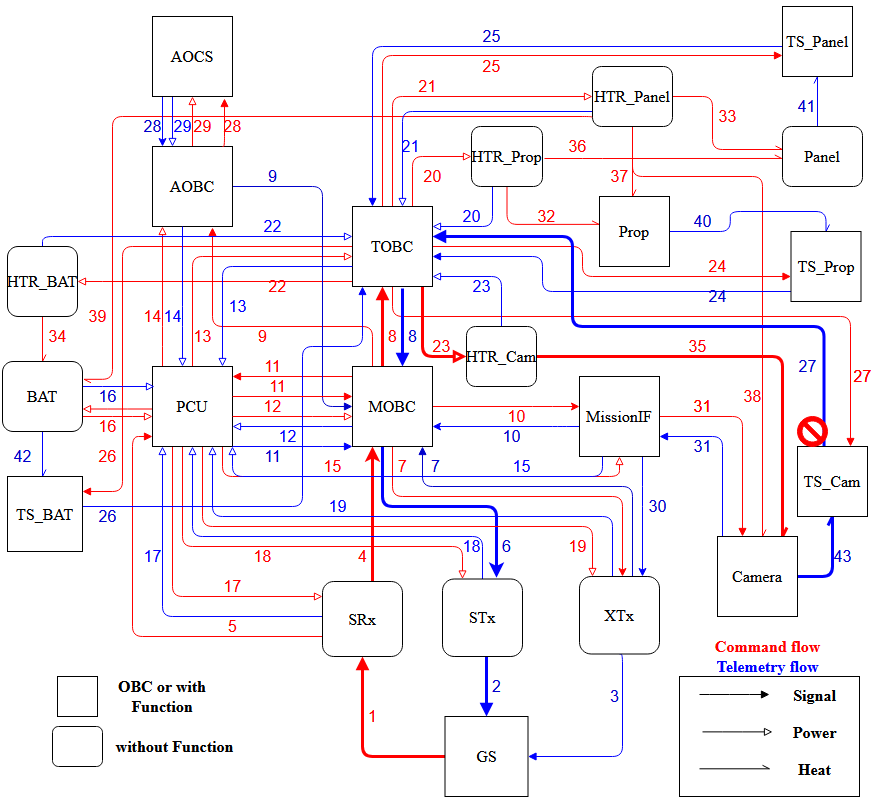
\includegraphics[height=13.0cm]{figure/fault_mode2.png}
      \caption{故障箇所:リンク24(推進系温度計-TOBC間)の時の故障候補}
      \label{fig:fault_mode2}
\end{figure}
この時,システムによって洗い出された検証用のコマンドは上の例(図\ref{fig:COM_candidate})
のものと同じであり,どちらのコマンドから検証を始めても結果は同じで以下の図\ref{fig:COM_process_TS_fault}
のようになった.
今回の不具合は温度計の断線であるため,パネルヒータによる推進系温度の変化も
推進系ヒータによる推進系温度変化も見ることはできないため,
提案されたコマンドによって推進系温度計に変化は見られず,異常テレメトリとなる.
そのため,どちらのコマンドによる検証でも切り分けを行うことができず,
故障箇所の特定を行うことができなかった.
このことから,この衛星の設計では今回扱った故障「(推進系)温度計故障」が発生した際に,
本手法を用いて故障特定を行えないことが分かる.\\

\begin{figure}[H]
   \centering
      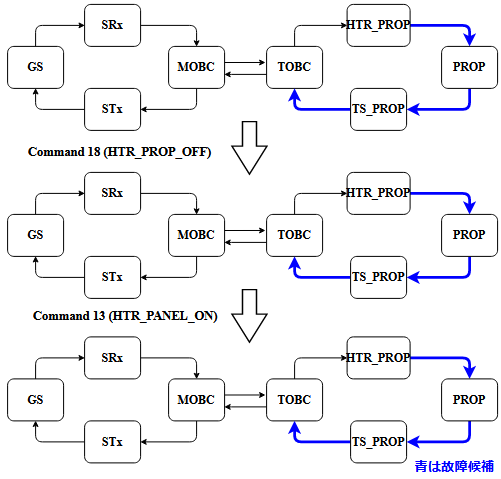
\includegraphics[height=8.0cm]{figure/COM_process_TS_fault.png}
      \caption{温度計故障時の検証の流れ}
      \label{fig:COM_process_TS_fault}
\end{figure}
一方で,不具合分析の過程で得た情報を用いた人間の推論を組み合わせることで故障箇所を
特定することは可能である.
まず,今回の事例では,TOBCから推進系ヒータへの電源供給ライン(コマンドリンク20)
が正常であることは「推進系ヒータ電流値」によって確認できており,
同時に「パネル温度」の上昇によってヒータが正常に作動していることも確認できるため,
推進系ヒータの故障ではないことが切り分けられる.\\
また,「パネルヒータON」によって推進系温度の変化を見ることができなかったことから,
「推進系−推進系温度計間」か「推進系温度計−TOBC間」のいずれかに確実に故障箇所があることが
推測できる.よって,温度計自体の故障か,TOBCの温度計読み取り回路のどれかが故障している
と判断することが可能である.\\
このように,本システムのみでは故障箇所の特定が行えなかった場合においても,
提示された選択肢に従って検証を行うことによって,
故障箇所を推論するために必要な情報が取得可能であることがわかる.


また,人間の推論を組み合わせても故障箇所の特定が行えなかった場合には,
設計の不備を考えることができる.衛星の地上試験及び軌道上での運用では,
基本的には本手法のようにコマンドとテレメトリでのやり取りによって人間との通信を行う.
そのため,これらの情報を用いて不具合分析が行えるような,コンポーネントの接続関係,
コマンドやテレメトリの設計を行う必要がある.
本手法を設計段階の衛星に対して適用することによって,衛星システムとして不具合発生時の
検証能力が十分であるかを確認することが可能である.\\
実ミッションでは,設計段階においてFMEA(Failure Mode and Effect Analysis)などを用いて,
衛星システムに起こりうる故障モードを列挙し,それらの故障モードによる影響や,
発見のしやすさなどを考え,設計の正しさを確認する.
この過程において,FMEA上で洗い出された
故障モードに対して本手法を適用することによって,それぞれの故障モードが発見可能な設計になっているか
を確認することができる.

%時間があれば
\section{本手法に関する考察}


\begin{comment}
まず,MOBCとTOBCからテレメトリは全て降ろされているものと仮定する.
また,故障は「推進系ヒータの接着不良」であるとする.
その時,テレメトリを通して確認できるのは
\begin{itemize}
   \item 「推進系ヒータON」コマンドを送ったのに,「推進系温度」テレメトリが変化しない.
\end{itemize}
という事象である.
よって不具合検知は,この事象によって行われる.

\subsection{不具合分析の例}
この不具合において,「推進系ヒータON」コマンドを送信して推進系ヒータに熱が伝わるまでの経路
と,推進系温度計が温度を読み取り「推進系温度」テレメトリとして地上局に伝わるまでの
経路の中に故障箇所があると考えることができる.
この経路を以下の図\ref{fig:simple_sat_fault}に太矢印で示している.
%これにリンクID入れたら見やすいかも
\begin{figure}[H]
   \centering
      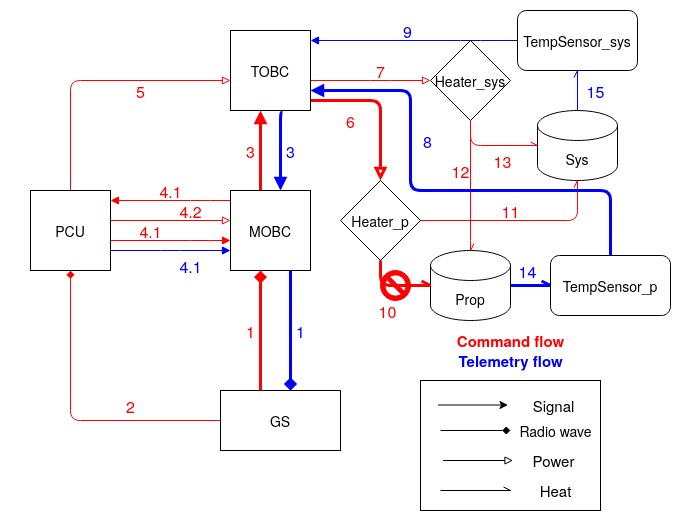
\includegraphics[height=9.0cm]{figure/simple_sat_fault.png}
      \caption{故障箇所と不具合検知に関連するコマンドとテレメトリの経路}
      \label{fig:simple_sat_fault}
\end{figure}
また,この経路内にあるコンポーネントに電源が入っているかどうかを確認するためには,
そのコンポーネントに電源を供給するための経路が正常に作動しているかどうかを確認する
必要がある.そこで
\begin{itemize}
   \item PCU$\rightarrow$MOBC(リンクID:4.2),PCU$\rightarrow$TOBC(リンクID:5)
\end{itemize}
も検証を行う対象として考える.
以上より,検証すべき経路は下記のようになる.
\begin{itemize}
   \item コンポーネント:GS,MOBC,TOBC,Heater\_p,Prop,TempSensor\_p
   \item コマンドリンク:GS-MOBC(1),MOBC-TOBC(3),MOBC-PCU(4.2),
   PCU-TOBC(5),\\TOBC-Heater\_p(6),Heater\_p-Prop(10)
   \item テレメトリリンク:GS-MOBC(1),MOBC-TOBC(3),TOBC-TempSensor\_p(8),
   TempSensor\_p-Prop(14)
\end{itemize}
以下,提案手法によるアルゴリズムによって不具合分析を行っていく.\\
%この章長くて読みにくい
まず,問題設定よりMOBC及びTOBCのテレメトリは全てダウンリンクされている状態に
あるので,
\begin{itemize}
   \item テレメトリリンク:TOBC$\rightarrow$MOBC(3),MOBC$\rightarrow$GS(1)
   \item コマンドリンク:PCU$\rightarrow$MOBC(4.2),PCU$\rightarrow$TOBC(5)
\end{itemize}
は問題ないことが確認できるため,故障可能性はなくなる.
問題設定ではあるが,実際に「MOBC及びTOBCのテレメトリが全てダウンリンクされている」
ことを確認するためには,「MOBCカウンター」
「TOBCカウンター」を確認することが必要である.\\
また不具合発生時,推進系ヒータが正常に作動しており,
システム温度計からテレメトリを下ろす経路に問題がなければ,
「システム温度」が上昇しているはずである.
よって,テレメトリの確認によって検証できる経路として,
コマンドリンク「TOBC-Heater\_p(6)」がある.
以上より,不具合発生時から状態変化させずに確認すべき事項として以下
が挙げられる.

\begin{table}[H]
   \centering
   \caption{コマンドなしでの確認事項} 
   \label{tab:check_list1}
\end{table}
\vspace{-2zh}
\begin{figure}[H]
   \centering
      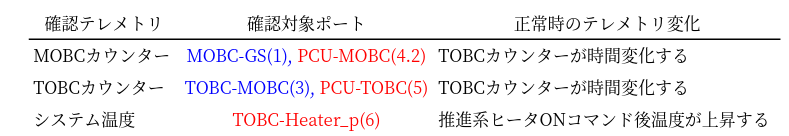
\includegraphics[height=2.5cm]{figure/check_list_tel.png}
\end{figure}
衛星の状態を変化させること無く,テレメトリを確認するだけで
検証できる箇所はこれ以上存在しないので,次にコマンドによる検証を行う.

まず,コマンドパスとしてGSに近い箇所から順に確認を行う必要がある.
MOBCへのコマンドが通っているかを確認するためには,「MOBCコマンドカウンターアップ」
コマンドを送って,「MOBCコマンドカウンター」が変化していることを確認できれば良い.
同様に考えると,以下の様に確認事項を洗い出すことができる.
\begin{table}[H]
   \centering
   \caption{コマンド送信による確認事項} 
   \label{tab:check_list2}
\end{table}
\vspace{-2zh}
\begin{figure}[H]
   \centering
      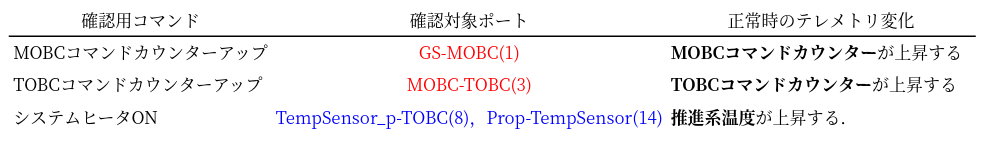
\includegraphics[height=2.6cm]{figure/check_list.png}
\end{figure}
以上の項目を確認した際,今回想定した故障モード(推進系ヒータの接着不良)
では期待されるテレメトリデータの変化が起こるので,
Table \ref{tab:check_list2}の確認対象パスの中にある故障可能性箇所は
棄却され,
故障可能性リンクとして残るのは
\begin{itemize}
   \item コマンドリンク:Heater\_p-Prop(10)
\end{itemize}
となる.

%上のコマンドを送っても大丈夫なのかという議論はどうするのか?もしシステム温度が高いのに,その方法でたしかめてもいいものなのか?

この経路上で考えうる故障モードと照らし合わせると,
この切り分けによって残る故障モードは
\begin{itemize}
   \item 推進系ヒータの故障
   \item 推進系ヒータの接着不良
\end{itemize}
となる.
この時,
「システム温度」の上昇によって「推進系ヒータの故障」の可能性は
棄却できるため,最終的に「推進系ヒータの接着不良」
が残り,
実際の故障を棄却すること無く,絞り込みができていると言える.\\
\end{comment}




\expandafter\ifx\csname ifdraft\endcsname\relax
  \end{document}
\fi
\expandafter\ifx\csname ifdraft\endcsname\relax
\documentclass[11pt]{report}
\usepackage{mypackage}
\begin{document}
\fi


\expandafter\ifx\csname ifdraft\endcsname\relax
  \end{document}
\fi
\expandafter\ifx\csname ifdraft\endcsname\relax
\documentclass[11pt]{jsreport}
\usepackage{mypackage}
\begin{document}
\fi

\chapter{結論}

\section{まとめ}
本研究では,衛星内の情報伝達経路モデルを用いてコマンドによる故障箇所特定の過程を
体系化する手法,及びコマンドの安全性と故障候補切り分け能力の大きさを示す指標
を提案した.
%手法に関するまとめ的なものを入れられたらいいのかもしれないなあ
また,本手法を簡易的な衛星モデルで仮想的に与えた故障状態に対して適用し,
本手法の評価を行った.\\
実践例では,複数のコマンドの中から故障箇所特定のために適切なコマンドを探索し,
そのコマンドに対して評価指標の計算を行ったものと共に提示した.
提示されたコマンドを用いて検証を行うことにより,想定した故障箇所を
特定できる能力があることを示した.\\
次に,コマンドの故障候補切り分け能力を示す指標に関して考察を行った.
そこでは,時間制約がより厳しい状況での不具合分析においては「平均確認可能性」の大きなコマンドを用いる
ことで数少ない通信の機会を利用できる可能性が高まること,
不具合分析に使用できる時間が明確に分かっており,ある程度の余裕がある場合には
「検証コマンド総数」が小さなコマンドを選択することで,最終的に少ない作業工程で
故障箇所の特定が行える可能性があることを示した.\\
%もう少し人との推論で特定できる,そのための情報を効率的に集めることができることを伝える.
また,故障状態によってはシステムのみでは特定を行えなかった場合があること
もわかった.そのような場合には人間の推論と組み合わせることで故障候補の絞り込みができ,
提示された選択肢に従うことで推論に必要な情報を効率的に得ることができることを示した.
同時に,人との推論を組み合わせても特定できない場合には設計の不備を考えられるため,
設計の不備を発見することにつながることを示した.

一方で,本手法では
安全性を示す指標として状態変化の小さなものが好ましいと考えていたが,
人による不具合分析結果との比較によって,実際は安全を確保するために状態変化をする場合がある
こと,本手法で見ることができる故障は主に接続関係に関するものに限定されており,
コンポーネントが持つ機能の故障まで特定することはできないことなどが知見として得られた.\\
これらを踏まえた今後の展望を次に示す.

%テレメトリを発行している機器の故障の場合は,そのコンポーネントから
%の情報ラインに冗長系がなければかなり多くの故障候補が残ってしまう.
%多分複数の検証結果を総合して判断するような処理が必要になるんやろな.これをシステム上で判断させること
%ができれば実現できるのかもしれないが,ムズいぜ
\newpage
  \section{今後の展望}
  今後取り組むべき課題として以下にまとめた.
\begin{itemize}
  \item コンポーネントの機能の接続関係を組み込んだ,より粒度の細かい故障箇所特定
  \item リンクの正常確率に実機の情報を組み込むことによる,検証の効率化
  \item 設計情報からのモデル自動生成
  %\item コマンドの安全性の評価・・・
  %\item 推論も
\end{itemize}
上記の課題に関して,今後進めていくべき具体的な取り組みを述べる.

まず,コンポーネントの接続関係の故障だけでなく,各コンポーネントの機能の故障
を扱うために,各コンポーネントが持つ機能の詳細なモデル化が必要になる.
コンポーネントの機能は,階層的になっておりある機能を満たすためのサブ機能が
存在するというような関係になっている.検証を行う過程に関しても
まずは粗い粒度で故障箇所の特定を行い,その後故障箇所コンポーネントの
持つ機能単位での故障の特定,サブ機能単位での故障の特定という風に段階的に
切り分けを行っていく必要があると考えている.\\
また,上述した機能に対する故障を見るためにはテレメトリが持つ情報の意味に関しても
システムが扱えるようなオントロジーを定義する必要がある.
現在,人間からの入力情報として,テレメトリが正常か異常かの2値しか与えることができていない.
実際には,テレメトリの種類によって正常か異常かの基準はいくつかあり,
 %このまとめ方も微妙な気がする.
\begin{itemize}
  \item[-] テレメトリの取得可否
  \item[-] テレメトリに含まれるパラメータの大小
  \item[-] テレメトリの変化の有無
\end{itemize}
などが考えられる.
これらの情報の違いを扱うために
「テレメトリの種別」という概念を導入し,人間による入力のパターンを増やすことで,
故障の種類を見分けることができるようにする必要がある.
また同時に,機能に対応した故障を特定するためには,テレメトリと状態量の対応付けを考える必要があり
このモデルをどのように構築するかに関しては今後検討を進めていく必要がある.\\

 また,本研究では各リンクの正常確率を簡単のため0.5と固定して与えた.
 実際の衛星開発では,その機関で長年培われた技術や,実績のある機器など信頼性の高い
 設計項目が存在し,同時に新規実装項目や開発途中のソフトウェアなど信頼性の低い設計箇所
 も存在するなど,ばらつきがある.そこで,
 リンクの正常確率を,実際に設計・製造している衛星の各設計項目に対する
 信頼度に基づいて考えることによって,より効率的な検証作業につながることが想像できる.
これらの信頼度は事前知識的に組み込むことは可能であるが,今後の課題としては
試験結果を元に不具合発生するコンポーネントの信頼性を下げていくなどし,学習させる
システムを構築することによって,対象とする衛星のモデルの再現度を高めることを検討したい.\\


また,本研究で用いた簡易的な衛星モデルは全て手作業によって記述した.
実際に開発される衛星では,超小型衛星であっても膨大な数のコマンド及びテレメトリ,%具体的な数ほしい
多くのコンポーネント間の回路などが存在し,手作業によるモデルの記述は作業コストや
ヒューマンエラーのリスクを考えると現実的ではない.また,実際の
開発過程においては設計変更が幾度に渡って繰り返されることがほとんどである.
そのため,その設計変更との整合性が取れなくなると本手法を用いた不具合分析を行うことは
不可能である.これらを踏まえると,設計情報からモデルを自動生成し,
設計情報の更新に応じて本手法で用いるモデルにも反映されるシステムが求められる.
設計情報の中には,各コンポーネントの電気回路の接続情報や,物理的位置関係
など,本手法で用いたモデルを構築するために必要な情報が含まれている.
それらの文書の中からモデル生成を行う手法に関して,検討していこうと考えている.



\begin{comment}
\section{まとめ}

%これも今後の展望かな??


%これも今後の展望かな
また,故障診断のコンテキストによってどこまで掘り下げるべきか使い分けるべきである
\cite{Ontology1998}ことを書く.

%モデルの波及効果に関してこれは今後の展望で述べるとこかな
一方で,人工衛星は内部のコンポーネントが非常に密集しているおり,人間が設計時に考慮した
意図したつながりだけでなく,意図しないつながりも多く存在する.
このような意図しないつながりによって,波及効果が発生することが衛星内部の理解が
困難になり
\end{comment}

\expandafter\ifx\csname ifdraft\endcsname\relax
  \end{document}
\fi
\expandafter\ifx\csname ifdraft\endcsname\relax
\documentclass[11pt]{report}
\usepackage{mypackage}
\begin{document}
\fi

\chapter*{謝辞}
本研究は多くの方々による支えによって書き上げることができました.
感謝申し上げます.

\expandafter\ifx\csname ifdraft\endcsname\relax
  \end{document}
\fi


%以下で何を書くかをまとめる
%まずは手法の説明
%モデルの説明
%コマンドを評価するための指標に関して
%探索のアルゴリズムの具体的説明???
%実装結果(できればわかりやすい形で示したい)
%探索結果に関する考察


\bibliographystyle{junsrt} %plain, acm, alpha とか
\bibliography{Ref} 
\end{document}